\chapter{Symetric cryptography}

\section[Задачі, напрямки та методи захисту інформації. Поняття про криптографічний захист інформації]{Лекція 1. Задачі, напрямки та методи захисту інформації. Поняття про криптографічний захист інформації}

\subsection{Області застосування, мета, методи захисту інформації}

На протязі свого існування людство пережило декілька інформаційних
революцій: створення і розвиток мов, винахід писемності, винахід та широке
застосування друкарства, створення комп’ютера та новітніх електронних
технологій, що радикально змінили суспільство в усіх галузях, на всіх рівнях
суспільного розвитку. Кількість інформації, що була доступна та
використовувалась, постійно зростала, а за періоди інформаційних революцій
– на декілька порядків. Володіння інформацією і в минулому і нині давало
можливість досягти швидкого розвитку і успіху у різних галузях як у
глобальному масштабі, так і в конкретних справах. Сьогодні світ переживає
період, коли накопичено колосальний об’єм знань, що дозволяє перейти до
здійснення справді революційних технологічних рішень. Основою розвитку
нині може бути, перш за все, процес пізнання, і він посильний тільки
високоосвіченому суспільству, в якому праця приймає все більш
інтелектуальні форми. Технологіям майбутнього потрібні широко освічені
люди, які здатні орієнтуватися в нових умовах дійсності, що стрімко
змінюється.
Однією з галузей, що найбільш динамічно змінюються протягом
останніх десятиліть, є технології електронної обробки інформації,
телекомунікацій, комп’ютерних мереж, технології захисту інформації.
В Україні широкий попит на методи і засоби захисту інформації почав
виявлятися у другій половині 80-х років ХХ ст. З часом виникла нагальна
потреба використання криптографічних та технічних методів захисту також у
приватному секторі. Сьогодні велика кількість конфіденційної інформації
передається в електронному вигляді, на електронних носіях, між ЕОМ
звичайними лініями зв’язку. Інформація може продаватися та купуватися,
мати ціну, що незрівнянно перевищує ціну матеріального носія. Часто
володіння інформацією дає переваги, ціну яких неможливо підрахувати,
наприклад, у військовій справі. Термін збереження секретності інформації
може коливатися від декількох годин до багатьох десятиліть. Тому вкрай
потрібні спеціалісти, які володіють криптографічними, технічними,
комплексними методами захисту, знають відповідні стандарти, здатні
використовувати (або розробляти) програмне й апаратне забезпечення для
гарантування таємності та цілісності конфіденційної інформації. 
Криптографічні методи захисту вважаються одними з найбільш надійних та
ефективних. 

\textbf{Області застосування захисту інформації (відповідно – види таємниці)}
\begin{enumerate}
    \item Військова;
    \item Дипломатична;
    \item Фінансова;
    \item Банківська;
    \item Комерційна;
    \item Промислова;
    \item Наукова;
    \item Юридична;
    \item Медична;
    \item Особиста таємниця.
\end{enumerate}

\textbf{Мета і головні задачі захисту інформації:}
\begin{enumerate}
    \item Конфіденційність (секретність) інформації;
    \item Цілісність інформації;
    \item Автентичність інформації;
    \item Доступність інформації;
    \item Спостереженність.
\end{enumerate}

\textbf{Напрямки, аспекти, методи і засоби захисту інформації:}
\begin{enumerate}
    \item Юридичні, правові;
    \item Методично-нормативні;
    \item Організаційні;
    \item Безпосередні (фізичні);
    \item Технічні - захист від витоку по технічним каналам:
        \begin{enumerate}
            \item електромагнітному;
            \item оптичному;
            \item акустичному;
            \item віброакустичному;
        \end{enumerate}
    \item Криптографічні методи захисту інформації;
    \item Стеганографічні;
    \item Методи кібербезпеки, захист кіберпростору;
    \item Методи квантової криптографії;
    \item Морально-етичні норми.
\end{enumerate}


\textbf{В сучасних умовах з точки зору реалізації криптографічні методи
можна поділити на:}
\begin{itemize}
    \item апаратні засоби,
    \item програмні засоби,
    \item програмно-апаратні засоби,
\end{itemize}

кожен з яких має свої переваги та недоліки. 

\subsection{Перші поняття криптографічного захисту інформації}

\begin{definition}[Криптографічний захист інформації]
    Криптографічний захист інформації – це різновид захисту
    інформації, який реалізується за допомогою криптографічних перетворень,
    спеціальних ключових даних з метою приховування та відновлення змісту
    інформації, підтвердження достовірності, авторства, запобігання
    несанкціонованому використанню тощо.
\end{definition}

\begin{definition}[Криптографічне перетворення]
    Криптографічне перетворення – це перетворення інформації
    відповідно до певних правил (логічних, математичних) з метою забезпечення
    функціонування криптографічних протоколів.
\end{definition}

\begin{definition}[Криптографічний ключ]
    Криптографічний ключ – це параметр, який використовується в
    криптографічному алгоритмі для вибору конкретного криптографічного
    перетворення; ключі можуть бути таємними або відкритими.
\end{definition}

\begin{definition}[Криптографічний протокол]
    Криптографічний протокол – це послідовність узгоджених дій
    згідно з деякими правилами, у відповідності з якими відбувається обмін
    інформацією між сторонами або учасниками протоколу та її перетворення з
    використанням криптографічних методів і засобів. Простий приклад
    криптографічного протоколу – це зашифрування та розшифрування
    повідомлення.
\end{definition}

\begin{definition}[Криптографія]
    Криптографія – науково-технічна дисципліна, яка вивчає принципи,
    методи і засоби криптографічного захисту інформації і інформаційних
    технологій, предметом якої є розробка криптографічних систем,
    забезпечення криптографічного захисту інформації.
\end{definition}

\begin{definition}[Криптоаналіз]
    Криптоаналіз – це науково-технічна дисципліна, яка вивчає методи,
    способи і засоби аналізу криптографічного захисту інформації:
    криптографічних систем, криптографічних алгоритмів, протоколів з метою
    знайти способи їх розкриття без знання секретних ключів і, можливо, будови
    криптосистем, знайти способи несанкціонованого доступу, підробки даних
    тощо. Криптоаналіз оцінює складність таких способів розкриття (злому) і
    стійкість криптографічного захисту інформації. Фахівця, який займається
    криптоаналізом будемо називати криптоаналітиком.
\end{definition}


Криптологія за найбільш поширеною сучасною термінологією,
об'єднує в собі дисципліни криптографію і криптоаналіз.

\begin{enumerate}
    \item Криптологія
    \begin{enumerate}
        \item Криптографія
        \item Криптоаналіз
    \end{enumerate}
\end{enumerate}

\begin{remark}
    Не всі країни дотримуються останньої термінології щодо
    дисциплін. Так, наприклад, в Росії назва „криптографія” об’єднує в собі
    власне криптографію (криптосинтез) у вище наведеному розумінні і
    криптоаналіз, а криптологія розглядається як галузь криптографії, що вивчає
    математичні моделі криптографічних систем, і також поділяється на
    криптосинтез та криптоаналіз.
\end{remark}

\begin{definition}[Алфавіт (абетка)]
    Алфавіт (абетка) – множина символів (букв), послідовностями яких
    записуються тексти. Будемо позначати:
    $$Z_m = \{z_1, z_2, ..., z_m\}, Z_m = \{z_0, z2, ..., z_m-1\} \text{ або } Z_m = \{0, 1, 2, ..., m-1 \}.$$
\end{definition}

\begin{definition}[Відкритий текст]
    Відкритий текст (ВТ) – повідомлення, дані, елемент простору
    повідомлень, до якого застосовується процедура криптографічного
    перетворення, шифрування. Звичайно, під ВТ розуміють текст, заданий у
    вигляді послідовності символів скінченого алфавіту, з доступним
    семантичним змістом. ВТ отримують після вірного розшифрування. ВТ
    записується послідовністю символів заданого алфавіту. Позначення ВТ:
    $$X = x_1, x_2, ..., x_n, \quad M = m_1, ..., m_n$$
\end{definition}

\begin{definition}[Шифрований текст]
    Шифрований текст, шифротекст або криптограма (ШТ) –
    інформація, яка отримана в після застосування до відкритого тексту
    процедури зашифрування. ШТ записується послідовністю символів певного
    алфавіту. Позначення ШТ:
    $$Y = y_1, y_2, ..., y_r, \quad C = c_1, c_2, ..., c_r$$
\end{definition}

\begin{definition}[Зашифрування]
    Зашифрування – криптографічне перетворення повідомлення, ВТ з
    застосуванням таємних ключів, в результаті якого буде отримано
    шифротекст або криптограму (ШТ) з недоступним для незаконного
    користувача семантичним змістом.
\end{definition}

\begin{definition}[Розшифрування]
    Розшифрування – зворотне криптографічне перетворення ШТ з
    застосуванням таємних ключів, в результаті цієї процедури законний
    користувач отримує ВТ, що був зашифрований. Використовують для даної
    процедури також термін дешифрування.
\end{definition}

\begin{definition}[Шифратор]
    Шифратор – пристрій, що здійснює процедуру зашифрування.
\end{definition}

\begin{definition}[Дешифратор]
    Дешифратор – пристрій, що виконує процедуру розшифрування.
\end{definition}

\begin{definition}[Криптографічна система]
    Криптографічна система – система забезпечення безпеки інформації
    криптографічними методами з використанням спеціальних математичних
    алгоритмів, криптографічних ключів, перш за все, для забезпечення
    конфіденційності, цілісності, автентичності, доступності. З практичної точки
    зору - це набір апаратних і (або) програмних засобів, інструкцій і правил, за
    допомогою яких, використовуючи криптографічні перетворення, можна
    зашифрувати повідомлення і розшифрувати криптограму різними способами,
    один із яких вибирається за допомогою секретного ключа, а також
    здійснювати інші криптографічні протоколи.
\end{definition}

\subsection{Етапи розвитку технологічних засобів криптографії}

\begin{enumerate}
    \item «Ручна» криптографія (із давнини до в основному початку XX
        століття). Основні види шифрів: шифри перестановки і шифри
        заміни.
        \begin{enumerate}
            \item Перший шифр перестановки, застосування якого зафіксоване у
            військовій справі, (Спарта, V ст. до н.е.) – шифр Скитала (рис. 1.1).
            Таємний ключ – діаметр барабана. 
    
            \begin{figure}[h]
                \centering
                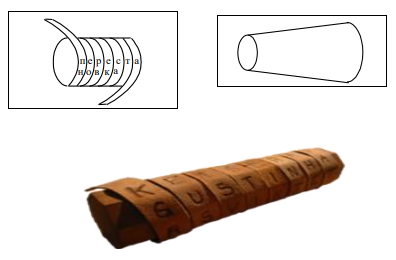
\includegraphics[width=5cm]{subjects/symcrypta/images/old_cryptographic_mashine.png}
                \caption{Шифр Скитала і засіб його криптоаналізу.}
            \end{figure}
            
            Для шифрування на стрічці, що намотувалась на барабан (скитал),
            писалось вздовж барабана повідомлення. Після знімання з барабану на
            стрічці була зовні випадкова послідовність літер – шифроване повідомлення.
            Криптоаналіз шифру Скитала запропонував Арістотель за допомогою
            барабана змінного діаметру (рис.1.1): якщо на намотаній на нього стрічці з
            шифрованим повідомленням у деякому місці вгадувались якісь частини слів,
            то цьому місцю відповідав діаметр справжнього барабану.
            
            \item Прикладом шифру заміни є шифр Цезаря – заміна кожної букви
            повідомлення на букву циклічно віддалену в алфавіті на фіксоване число
            позицій.
        \end{enumerate}
    \item Застосування телеграфу для шифрування і кодування
        (з середини XIX ст.).
    \item Використання механічних машин (кінець XIX ст. – початок XX ст.).
    \item Електромеханічні машини (з 20-х років XX ст. – друга половина XX
        ст. ). Приклад – ENIGMA – основна шифрувальна машина Вермахту у Другій
        світовій війні.
    \item Електронні машини (з кінця 40-х років XX ст.).
    \item Напівпровідникові криптосистеми.
    \item Криптосистеми, засновані на мікросхемах.
    \item Використання комп'ютерної техніки для криптографічного захисту.
    \item Квантова криптографія.
\end{enumerate}

\subsection{Про розвиток теоретичної криптографії}

До епохи Відродження криптографією займалися, можна сказати, не
професіонали. Найчастіше шифри уявляли собою деякі головоломки. Але
слід зазначити, що іноді винаходилися шифри, які не були розкриті на
протязі 100 і навіть більше років! Хоча за сучасними поняттями,
враховуючи залучення до криптоаналізу ЕОМ, загалом це були слабкі,
нестійкі шифри.

Велике просування в криптографії відбулося після залучення до
вирішення її проблем відомих математиків періоду відродження, серед яких
були Ф. Вієт, Д. Кардано та ін. Пізніше почали створюватись спеціалізовані
державні служби шифрування і дешифрування (розкриття). Такі служби
створили, наприклад, Кромвель у Англії, кардинал Рішельє у Франції, Петро
I в Росії.

У 1883 році була опублікована книга Керкгоффа «Військова
криптографія», в якій були вперше сформульовані деякі вимоги до
криптосистем, правила щодо утворення, експлуатації, стійкості
криптографічних пристроїв. Частина цих правил і зараз вважаються
обов'язковими. Наукою у повному розумінні цього слова теоретичну
криптографію стали визнавати з 1949 року після публікації у відкритому
друці статті К. Шеннона «Теорія зв'язку в секретних системах».

А з 1976 року завдяки ідеям статті Діффі і Хеллмана «Нові напрямки в
криптографії» почався новий етап у розвитку криптографії – застосування
асиметричних криптосистем з відкритим ключем, яке дало можливість
успішно вирішити низку назрілих проблем криптографічного захисту
інформації.

В 1983 криптографи Беннет і Брассар запропонували використовувати
для захисту інформації квантові властивості мікрочастинок. Перша реалізація
квантової передачі здійснена в 1989 році. Виник новий напрям в захисті
інформації – квантова криптографія.

\subsection{Класифікація криптосистем і напрямків криптографії}

\begin{enumerate}
    \item Симетричні криптосистеми (одноключові, з секретним ключем).
        У відправника та одержувача повідомлення один і той самий секретний
        ключ, вони знаходяться у рівних (симетричних) умовах, можуть як
        зашифрувати повідомлення так і розшифрувати за допомогою
        таємного ключа.
        
        Підрозділяються на:
        \begin{itemize}
            \item класичні шифри (шифри ручної криптографії),
            \item сучасні криптосистеми:
                \begin{itemize}
                    \item блокові криптосистеми,
                    \item потокові криптосистеми.
                \end{itemize}
        \end{itemize}

        \item Асиметричні криптосистеми (двохключові, з відкритим ключем, із
            загальнодоступними ключами).
            
            У найпростішому випадку мають два ключі: один відкритий – у
            відправників, інший – секретний у одержувача. Зашифрування
            повідомлення виконується з допомогою відкритого ключа (будь ким), а
            розшифровується криптограма тільки з використання секретного
            ключа. Відомі з 1976 року, активно використовуються на практиці з
            1978 року.
        
        \item Квантові криптосистеми (з 1983 р., знаходяться у стадії
            експерименту та розвитку).
\end{enumerate}

\textbf{Відповідно маємо такі напрямки криптографії.}

\begin{enumerate}
    \item Симетрична криптографія:
        \begin{itemize}
            \item класична криптографія,
            \item сучасна криптографія.
        \end{itemize}
    \item Асиметрична криптографія.
    \item Квантова криптографія.
\end{enumerate}

\subsection{Контрольні питання}
\begin{enumerate}
    \item Які мета та задачі захисту інформації?
    \item Назвіть напрямки та методи захисту інформації.
    \item Що таке криптографічний ключ?
    \item З яких частин складається криптологія?
    \item Чи були відомі способи захисту інформації шифруванням до нашої ери?
    \item Коли використовувались роторні шифрувальні машини?
    \item Яка дата вважається початком розвитку криптографії з відкритим ключем?
    \item Чим відрізняються симетричні криптосистеми від асиметричних?
\end{enumerate}

\section[Моноалфавітні підстановки і блокові шифри]{Лекція 2. Моноалфавітні підстановки і блокові шифри}


\subsection{Моноалфавітні підстановки. Загальний шифр простої заміни}

Нехай $\mathbb{Z}_m = \{z_1, z_2, ..., z_m\}$ --- алфавіт відкритого та шифрованого текстів.

\begin{definition}[Підстановка на алфавіті $\mathbb{Z}_m$]
    Підстановкою на алфавіті $\mathbb{Z}_m$ називається взаємнооднозначне відображення
    $$\pi : \mathbb{Z}_m \rightarrow \mathbb{Z}_m$$
\end{definition}

Підстановку на алфавіті можна задати таблицею, наприклад,

\begin{table}
\centering
% \tiny
\begin{tabular}{|c|c|c|c|c|c|c|c|c|c|c|c|c|c|c|c|c|}
    \hline А & Б & В & Г & Ґ & Д & Е & Є & Ж & З & И & І & Ї & Й & К & Л & М  \\
    \hline У & П & Ь & Х & Ж & К & Г & И & Ш & Я & С & Н & Д & Р & Ц & О & Т  \\
    \hline
\end{tabular}
\end{table}

\begin{table}
\centering
% \footnotesize
\begin{tabular}{|c|c|c|c|c|c|c|c|c|c|c|c|c|c|c|c|}
    \hline Н & О & П & Р & С & Т & У & Ф & Х & Ц & Ч & Ш & Щ & Ь & Ю & Я  \\
    \hline Б & Е & Ю & Й & Ї & Ґ & Ф & А & Ч & Щ & І & М & З & Є & Л & В  \\
    \hline
\end{tabular}
\end{table}


У першому рядку підстановки $\pi$ розташований алфавіт, у другому може
бути будь-яка перестановка букв алфавіту. Ця перестановка елементів $\mathbb{Z}_m$ у
другому рядку визначає підстановку на $\mathbb{Z}_m$. Кількість всіх підстановок на
$\mathbb{Z}_m$ дорівнює $M!$.

Якщо задана підстановка $\pi$ на $\mathbb{Z}_m$, то можна згідно з нею кожній букві
ВТ співставити букву ШТ. Так, у нашому прикладі буква А відкритого тексту
буде замінена буквою У в ШТ, буква Б перейде при шифруванні в букву П і
т.д.

\begin{definition}[Шифр моноалфавітної підстановки]
    Шифром моноалфавітної підстановки називається
    спосіб шифрування ВТ в алфавіті Шифром моноалфавітної підстановки, при якому кожна буква ВТ замінюються
    на іншу однією підстановкою $\pi$ на алфавіті Шифром моноалфавітної підстановки, яка і є секретним ключем для
    зашифрування і розшифрування.
\end{definition}

Для розшифрування більш зручніше використовувати секретний ключ у
вигляді оберненої підстановки $\pi^{-1}$, яка легко отримується
з підстановки $\pi$.

Якщо ж при шифруванні заміною на різних позиціях використовується
більше однієї підстановки на алфавіті (тобто букви ВТ можуть шифруватися
різними підстановками на алфавіті в залежності від їх місця у ВТ), то таке
криптографічне перетворення називається \textbf{поліалфавітною підстановкою}
(див. лекцію 3).

Підкреслимо, що при моноалфавітній підстановці одна й та сама буква
алфавіту, що зустрічається у ВТ, при шифруванні замінюється тією ж самою
буквою незалежно від її місця у тексті. Наприклад, якщо підстановка $\pi$
переводить букву „а” в букву „м”, то де б не зустрілась буква „а” у ВТ, вона
буде зашифрована як „м”. У разі ж поліалфавітної підстановки одна й та сама
буква алфавіту може шифруватись по-різному в залежності від її місця у ВТ.

\begin{definition}[шифр простої заміни]
    \textbf{Загальна моноалфавітна підстановка}, для якої
    секретним ключем може бути будь-яка підстановка $\pi$ на алфавіті $\mathbb{Z}_m$ і
    потужність ключового простору $|\mathcal{K}| = m!$, називається \textbf{шифром простої
    заміни}.
\end{definition}

Потужність ключового простору є важливішою характеристикою шифру.
Якщо, наприклад, ВТ є текстом природної мови, то, як правило, інформації в
криптограмі цього тексту достатньо, щоб знайти секретний ключ і ВТ
\textbf{методом повного перебору} (інакше грубої сили). Метод полягає в переборі
всіх ключів, розшифрування ШТ кожним поки не буде отримано змістовний
текст. Тому кількість можливих ключів повинна бути такою, щоб такий
перебір був неможливим навіть з застосуванням суперкомп’ютерів. Переважна
більшість шифрів мають обмежене число ключів і мистецтво та наука
побудови практично стійких криптосистем полягає у створенні таких шифрів,
для яких не існувало б методу зламу кращого ніж метод повного перебору,
принаймні суттєво кращого.

Для шифру простої заміни кількість ключів для латинського алфавіту
дорівнює $m! = 26! \approx 4 \cdot 10^{26}$, для кирилиці (якщо вважати, що алфавіт
складається з 32 букв) - $m! = 32! \approx 2.6 \cdot 10^{35}$. При цьому ключі мають бути
незалежними і рівномірно розподіленими на просторі усіх ключів. Якщо ж в
якості ключів брати, наприклад, змістовні тексти, то кількість ключів різко
скоротиться, що призведе до критичного зниження стійкості криптосистеми.
Кількість ключів шифру простої заміни, як бачите, така, що криптоаналіз
перебором по ключам «грубою силою» неможливий і з застосуванням
комп’ютерів. Та тут існують і більш швидкі методи.

Загальний шифр простої заміни є яскравим прикладом шифру, який
незважаючи на досить великий ключовий простір, піддається криптоаналізу,
хоча й не так легко, як більш прості історичні шифри моно алфавітної
підстановки.

Знаходження однієї вірної пари $x \leftrightarrow y$
мало що дає для розшифрування
тексту. Потрібно знаходити відповідності серед кількох найбільш частих
букв ВТ і ШТ, а також найменш частих букв. Крім того, існує багато
прийомів криптоаналізу, що межують з мистецтвом. Можна, наприклад,
визначити біграми, які часто зустрічаються у мові, а біграми зворотного 
порядку – рідко (в англійській мові це, наприклад, ТН – НТ, НЕ – ЕН), а
також біграми, що мають велику і приблизно однакову частоту в прямому і
зворотному порядку (RE – ER), і шукати відповідні за частотою біграми ШТ.

Якщо є підстави припустити, що деяке слово неодноразово
зустрічається в тексті, можна шукати відповідну послідовність букв у ШТ (це
особливо ефективно, коли в слові повторюються букви). Цей метод має назву
\textbf{методу вірогідного слова}. Існує також багато інших прийомів.

Таким чином, моноалфавітна підстановка піддається криптоаналізу,
тому що вона зберігає \textbf{статистичні властивості} мови --- частоти
букв, біграм, слів і т.д.

\begin{definition}[Частотний аналіз]
    Метод криптоаналізу, що базується на порівнянні
    частот букв, біграм, слів і інших елементів тексту у ШТ і в мові, якою
    написаний ВТ, називається частотним аналізом.
\end{definition}

Чим ближчий розподіл букв у ВТ до рівномірного, тим складніше
застосовувати частотний аналіз. Тому, як правило, ВТ перед шифруванням
піддають деякому перетворенню, що згладжує нерівномірність частот. Так,
наприклад, видаляють пробіл, що є найчастішою «буквою» алфавіту.

\subsection{Приклади історичних шифрів моноалфавітної підстановки}

Розглянемо історичні шифри моноалфавітної підстановки, які були більш
простими ніж загальний шифр простої заміни, з більш простим частотним
криптоаналізом, але більш зручними при «ручному» шифруванні.

\subsubsection{Шифр Цезаря}

Найпростіша моноалфавітна підстановка – це шифр Цезаря.
Ототожнимо букви алфавіту $\mathbb{Z}_m$ з числами від $0$ до $m-1$ і позначимо через $x$
довільну букву ВТ, а через $y$ – відповідну букву ШТ.

В шифрі Цезаря шифрування відбувається заміною кожної букви на
букву, яка стоїть в алфавіті на $b$ кроків попереду,
$1 \leqslant b \leqslant m-1$. Число $b$ є
\textbf{секретним ключем} шифру, а число всіх можливих ключів (потужність
ключового простору) $|\mathcal{K}| = m-1$. При зашифруванні і розшифруванні зручно
використовувати математичний запис і такі формули.

\textbf{Зашифрування} в шифрі Цезаря виконується за правилом
$$y = x + b (\mod m),$$

де $b$ --- \textbf{секретний ключ}, $1 \leqslant b \leqslant m-1$.

\textbf{Розшифрування} в шифрі Цезаря виконується за правилом
$$X = y - b (\mod m)$$

Сам Цезар використовував ключ $b=3$. В цьому випадку другий рядок
підстановки $\pi$ на алфавіті є циклічним зсувом алфавіту на
$b$ позицій вліво.

\textbf{Криптоаналіз шифру Цезаря}. В прикладі криптоаналізу шифру Цезаря
продемонструємо ідею частотного криптоаналізу. Для того, щоб знайти
ключ, маючи лише ШТ, використаємо частоти стрічання однакових букв в
шифрованому тексті. Знайдемо $y^{*}$ --- букву, що найчастіше зустрічається у
ШТ. Нехай $x^{*}$ --- буква алфавіту, що має найбільшу частоту у мові, якою
написаний ВТ. Тоді, якщо текст достатньо довгий, щоб у ньому проявилися
закономірності мови, найвірогідніше, що $x^{*}$ зашифровано у $y^{*}$. Отже,
маємо $y^{*} = x^{*} + b (\mod m)$, звідки ключ $b = y^{*} - x^{*} (\mod m)$.

Звичайно, існує деяка імовірність помилки при виборі образу $x^{*}$, а отже,
і при визначенні ключа $b$. Тоді потрібно взяти другу за частотою букву ШТ
$y^{**}$ і спробувати ключ $b = y^{**} - x^{*} (\mod m)$ і т.д., доки не одержимо
змістовний текст.

Справді, шифр Цезаря можна легко зламати і повним перебором ключів.
На шифрі афінної підстановки, біграмної афінної підстановки, як ми
побачимо далі, вже відчувається наскільки частотний аналіз може працювати
краще методу повного перебору.

\subsubsection{Шифр афінної підстановки}

У шифрі Цезаря ключ може приймати всього m-1 значень, де m –
потужність алфавіту. Оскільки m невелике, то всі ключі можна досить
швидко перебрати, інакше кажучи, шифр Цезаря має малий ключовий
простір. Розглянемо трохи складніший шифр --- \textbf{шифр афінної підстановки}.

\textbf{Защифрування} в шифрі афінної підстановки виконується за правилом
\begin{equation}
    \label{affine_substitution_cipher}
    y = ax + b (\mod m)
\end{equation}
 
\textbf{Секретний ключ}: пара чисел $(a, b)$, $1 \leqslant a \leqslant m-1$,
$0 \leqslant b \leqslant m-1$, причому $a$
повинно бути взаємно простим з $m$. З \ref{affine_substitution_cipher}
одержуємо алгоритм розшифрування.

Розщифрування в шифрі афінної підстановки виконується за правилом
\begin{equation}
    \label{affine_substitution_decipher}
    x = a^{-1} (y-b) (\mod m)
\end{equation}

д $a^{-1} \mod m$ --- обернений до $a$ елемент в кільці лишків за модулем $m$.


\textbf{Потужність ключового простору} $|\mathcal{K}| = m \varphi(m)$, де
$\varphi(m)$ --- функція Ойлера --- кількість чисел
від $1$ до $m$, які взаємно прості з $m$. Ця важлива
характеристика шифру значно більша ніж в шифрі Цезаря.

Рівність \ref{affine_substitution_decipher} має той самий вигляд,
що й \ref{affine_substitution_cipher}, отже шифрування і
розшифрування здійснюються за однаковим алгоритмом, тільки з різними
параметрами. Умова взаємної простоти $a$ з $m$ потрібна для того, щоб існував
обернений елемент $a^{-1}$ і рівняння \ref{affine_substitution_cipher}
при фіксованому $y$ мало розв’язок $x$ і
цей розв’язок єдиний. Тоді можливо однозначне розшифрувати ШТ. У
противному випадку рівняння \ref{affine_substitution_cipher}
має не єдиний розв’язок $x$ або взагалі
його не має.

\textbf{Криптоаналіз афінної підстановки}. Афінна підстановка теж легко
піддається частотному криптоаналізу, хоча кількість ключів в цьому шифрі
значно більша, ніж у шифрі Цезаря, а саме $\varphi(m) \cdot m$.

Нехай $y^{*}$ і $y^{**}$ --- перша і друга за частотою букви ШТ,
$x^{*}$ і $x^{**}$ --- відповідно найчастіша і наступна за нею
за частотою букви мови.

Природно припустити, що при шифруванні $x^{*}$ перейшла в $y^{*}$, а
$x^{**}$ --- в $y^{**}$.

Складемо систему рівнянь:
\begin{equation}
    \label{cryptanalysis_of_affine_substitution}
    \left\{ \begin{array}{l}
        y^{*} = a x^{*} + b \mod m \\
        y^{**} = a x^{**} + b \mod m \\
    \end{array} \right.
\end{equation}

Відмітимо, що в цій системі невідомими є $a$ і $b$, а $x$ і $y$ – відомі.

З \ref{cryptanalysis_of_affine_substitution} маємо:
\begin{equation}
    \label{equation_cryptanalysis_of_affine_substitution}
    y^{*} - y^{**} = a(x^{*} - x^{**}) \mod m
\end{equation}

Якщо пари $x^{*} \leftrightarrow y^{*}$, $x^{**} \leftrightarrow y^{**}$
підібрані вірно, то рівняння \ref{equation_cryptanalysis_of_affine_substitution} має
розв’язок $a$. Знаючи $a$, з \ref{cryptanalysis_of_affine_substitution} знаходимо
$b$. Якщо ж ці пари не відповідають дійсності, то
\ref{equation_cryptanalysis_of_affine_substitution} або не має
розв’язку, або при всіх розв’язках \ref{cryptanalysis_of_affine_substitution}, 
розшифровуючи, одержимо беззмістовний текст. Тоді можна розглянути
пари $x^{*} \leftrightarrow y^{**}$, $x^{**} \leftrightarrow y^{*}$
або деякі інші пари серед невеликої кількості найчастіших букв ШТ і ВТ.

\subsubsection{Шифри моноалфавітної заміни з різними алфавітами ВТ і ШТ}

Використовують також різні алфавіти ВТ $\mathbb{Z}_m$ і ШТ $\mathbb{Z}_r$, які мають різні
символи і не обов’язково природної мови, причому Секретним ключем
і правилом заміни букв ВТ є ін’єктивне відображення $K: \mathbb{Z}_m \rightarrow \mathbb{Z}_r$.

\textbf{Шифр таблиця Енея (Спарта)}. ШТ --- нитка з відмітками (наприклад,
вузлами), яка намотувалася для зашифрування на тверду табличку з алфавітом,
записаним в одну лінію. Відмітки на нитці (наприклад, вузли) ставилися
послідовно з кожним обертом нитки в місці, яке відповідало букві ВТ.
Розмотана нитка з вузлами і була ШТ. Секретним ключем є табличка з
алфавітом (її розмір, відстань між буквами та можливо порядок запису букв).
Для розшифрування нитка з вузлами намотувалася на табличку з алфавітом і
на кожному оберті вузол вказував на чергову букву ВТ. Алфавітом
шифрованого тесту тут були відстані від початку таблички до кожної букви.

\textbf{Шифр Полібія (Греція)}. Нехай ВТ представлено в латинському
алфавіті. Алфавіт записується в таблицю або в порядку слідування букв в
алфавіті, або за допомогою \textbf{ключового слова, яке є секретним ключем},
і пишеться спочатку. Далі записують букви алфавіту, що не входять у ключове
слово, в алфавітному порядку. Наприклад, якщо в латинському алфавіті
об’єднати букви I та J і вибрати ключовим словом „LIBERTY”, то таблиці
шифрування в першому і другому випадку будуть мати вигляд (відповідно
зліва і справо):


$$\begin{matrix}
    \begin{bmatrix}
        A & B & C & D & E  \\
        F & G & H & I & K  \\
        L & M & N & O & P  \\
        Q & R & S & T & U  \\
        V & W & X & Y & Z  \\
    \end{bmatrix}
    &
    \begin{bmatrix}
        L & I & B & E & R  \\
        T & Y & A & C & D  \\
        F & G & H & K & M  \\
        N & O & P & Q & S  \\
        U & V & W & X & Z  \\
    \end{bmatrix}
\end{matrix}$$

При шифруванні кожна буква ВТ замінюється на її координати в таблиці:
числові (наприклад, букві S відповідатиме впорядкована пара (4,3)) або за
допомогою інших символів.

\textbf{«Тюремний» шифр}. Це фактично шифр Полібія, в якому координати букви
передавалися звуковими сигналами, наприклад, перестуковунням, або
світовими сигналами.

\subsection{Шифри моноалфавітної підстановки в розширених алфавітах. Блокове шифрування.}

Узагальненням шифру моноалфавітної підстановки можна вважати
шифри, у яких текст розбивається на $n$-грами (блоки) і ключем є підстановка
на множині всіх $n$-грам. Тоді потужність ключового простору для шифру
простої заміни буде $|\mathcal{K}| = m^{n}!$, коли алфавіт ВТ $\mathbb{Z}_m$.

Часто ВТ розбивають на біграми і в якості алфавіту розглядають
множину біграм. Алфавіт тут значно більший і частотний криптоаналіз
вимагає шифрованих текстів суттєво більшої довжини. Прикладами таких
шифрів є афінна підстановка біграм, а також шифр Плейфера.

\subsubsection{Шифр Плейфера}

Букви алфавіту розміщують у квадратній таблиці $n \times n$. Якщо кількість
букв у алфавіті не є повним квадратом, то деякі букви об’єднуть або до
алфавіту додають символи. Таблицю заповнюють по рядках: спочатку
пишуть \textbf{ключове слово, яке є секретним ключем} може мати довжину $k$ від $1$
до $n^2$. Далі записують букви алфавіту, що не входять у ключове слово, в
алфавітному порядку. Наприклад, якщо в латинському алфавіті об’єднати
букви I та J і вибрати ключовим словом „LIBERTY”, то квадрат Плейфера
буде мати вид:

$$\begin{matrix}
    L & I & B & E & R  \\
    T & Y & A & C & D  \\
    F & G & H & K & M  \\
    N & O & P & Q & S  \\
    U & V & W & X & Z  \\
\end{matrix}$$

Якщо у ключовому слові деякі букви повторюються, то залишають
тільки першу з однакових букв. Наприклад, якщо ключем є слово
\textbf{PLAYFAIR}, то на початку заповненння таблиці будуть
записані букви \textbf{PLAYFIR}.

При шифруванні ВТ розбивається на біграми, що не перетинаються.
Попередньо між буквами, що повторюються, вставляють деяку букву, яка
має малу частоту і ніколи не зустрічається двічі підряд, наприклад
\textbf{Q}. Тобто замість слова, скажімо, \textbf{BUTTER} треба записати
\textbf{BUTQTER}, а замість слів \textbf{SENT TO} --- \textbf{SENTQ TO}.
Отже, при розбитті на біграми не зустрінеться біграма з двох однакових
букв. Можна замість \textbf{Q} використати деякий спеціальний символ,
ввівши його до алфавіту.

Кожна біграма ВТ шифрується таким чином:
\begin{itemize}
    \item якщо букви біграми стоять в одному рядку, то відповідна біграма ШТ
    складається з букв, що стоять в тому ж рядку справа від даних. При
    цьому вважається, що перший стовпчик стоїть справа від останнього.
    Наприклад, біграма YC зашифрується як AD, а біграма FM – як GF;
    \item якщо букви біграми стоять в одному стовпці, то вона шифрується
    біграмою, що складається з букв, які стоять в тому ж стовпці під
    даними; при цьому вважається, що перший рядок знаходиться під
    останнім;
    \item якщо букви біграми стоять у різних рядках і стовпцях, то відповідна
    шифрована біграма складається з букв, що стоять у протилежних кутах
    прямокутника, заданого даними буквами. Наприклад, біграма TQ буде
    зашифрована як СN.
\end{itemize}

Розшифрування ШТ законним користувачем виконується побіграмно в
оберненому порядку.

Шифр Плейфера можна розглядати як моноалфавітну підстановку над
алфавітом, який є множиною всіх біграм.

Якщо фіксувати довжину ключа $n$, то кількість \textbf{ключів у шифрі
Плейфера} дорівнює
$$|\mathcal{K}|
= A_{n^2}^k
= n^2 (n^2 - 1) (n^2 - 2) ... (n^2 - k + 1).$$

А максимально можлива кількість ключів дорівнює $n^2!$, тобто така як у
шифру простої заміни над алфавітом з $n^2$ символів (але деякі з них при
шифруванні коротких ВТ можуть будуть еквівалентними, тобто однаково
шифрувати однакові ВТ).

Шифр Плейфера також піддається \textbf{частотному аналізу}, хоча й дуже
клопіткому. При криптоаналізі використовують як частоти біграм, так і деякі
обмеження і закономірності, що випливають з правил шифрування.

\begin{remark}
    Для реалізації шифру Плейфера можна використовувати
    не тільки квадратні, а й прямокутні таблиці для запису символів алфавіту. 
\end{remark}

\subsubsection[Шифр н-грамної афінної підстановки]{Шифр $n$-грамної афінної підстановки}

Розглянемо узагальнення шифру афінної підстановки. Нехай відкритий і
зашифрований тексти задані в алфавіті $\mathbb{Z}_m$. Відкритий текст
$$X = x_1 x_2 ... x_n x_{n+1} ... x_{2n} x_{2n + 1} ...$$

розбивається на блоки по $n$ символів. Запишемо шифрований текст теж у
вигляді послідовностей блоків
$$Y = y_1 y_2 ... y_n y_{n+1} ... y_{2n} y_{2n + 1} ...$$

При шифруванні кожен блок ВТ перетворюється у відповідний блок ШТ.

Розглянемо процес \textbf{шифрування} на прикладі 1-го блоку. Кожному з
$m^n$ варіантів 1-го блоку ВТ $x_1 x_2 ... x_n$ поставимо у відповідність його номер
$X_1$, $0 \leqslant X_1 \leqslant m^n - 1$. Зручно впорядкувати вектори
$x_1 x_2 ... x_n$ в лексикографічному порядку. Алфавіт запишемо у вигляді
$\mathbb{Z}_m = \{0, 1, 2, ..., m - 1\}$. Тоді
$$X_1 = x_1 m^{n-1} + x_2 m^{n-2} + ... + x_{n-1} m + x_n.$$

Аналогічно номер 1-го блоку ШТ $y_1 y_2 ... y_n$
$$Y_1 = y_1 m^{n-1} + y_2 m^{n-2} + ... + y_{n-1} m + y_n.$$

\textbf{Секретним ключем} $n$-грамної афінної підстановки є пара чисел $(a, b)$,
$0 \leqslant a \leqslant m^n - 1$, $0 \leqslant b \leqslant m^n - 1$ , причому $a$
повинно бути взаємно простим з $m^n$ для існування $a^{-1} (\mod m^n)$.
\textbf{Потужність ключового простору} дорівнює
$|\mathcal{K}| = m^n \varphi(m^n)$.

\textbf{Шифрування проходить за формулою}
$$Y_1 = a X_1 + b(\mod m^n).$$

Номер $Y_1$ блоку ШТ розписується як послідовність відповідних букв
$y_1 y_2 ... y_n$, яка є записом числа $Y_1$ в позиційній системі
числення з основою $m$.

\textbf{Розшифрування} законним користувачем виконується за формулою
$$X_1 = a^{-1} (Y_1 - b) (\mod m^n)$$

і номер $X_1$ блоку BТ розписується як послідовність відповідних букв
$x_1 x_2 ... x_n$, яка є записом числа $X_1$ в позиційній системі
числення з основою $m$.

При $n = 1$ маємо шифр моноалфавітної афінної підстановки. При
$n = 2$ отримаємо шифр біграмної афінної підстановки.

\textbf{Для частотного аналізу} $n$-грамної афінної підстановки (аналогічно як
для частотного аналізу моноалфавітної афінної підстановки) по двом
найбільш частим $n$-грамам ШТ і двом найбільш частим $n$-грамам мови
будується система з двох рівнянь за модулем $\mod m^n$ відносно двох
невідомих параметрів ключа $(a, b)$. Але зауважимо, що для $n > 4$ для
проведення такого частотного криптоаналізу потрібно мати практично
нереально великі шифровані тексти.

\textbf{Підкреслимо}, що шифр $n$-грамної афінної підстановки є фактично
моноалфавітною підстановкою над алфавітом, який є множиною всіх $n$-грам.

\subsubsection{Шифр Хілла}

Можна узагальнити шифр афінної підстановки на підстановки $n$-грам
іншим способом, який має назву шифру Хілла, або шифрування за Хіллом.
Нехай відкритий і зашифрований тексти задані в алфавіті $\mathbb{Z}_m$. ВТ
і ШТ розбиваються на $n$-грами, як в шифрі $n$-грамної афінної підстановки, і
розглядаються як послідовності $n$-вимірних векторів над кільцем лишків $\mathbb{Z}_m$.

\textbf{Секретним ключем шифру Хілла} є пара $(A, \overline{b})$, де
$A$ --- невироджена матриця $n \times n$, а $\overline{b}$ --- довільний
вектор довжини $n$ над $\mathbb{Z}_m$. Всі операції над
елементами виконуються за $\mod m$. Перевірку невиродженності матриці $A$
можна виконати за такими твердженнями.

\begin{claim}
    Твердження 2.1.
    A --- невироджена $(n \times n)$ --- матриця над кільцем $\mathbb{Z}_m$ тоді і
    тільки тоді, коли $\det A = |A|$ взаємно простий з $m$, $(|A|, m) = 1$.
\end{claim}

\begin{claim}
    $A$ --- невироджена $(n \times n)$ --- матриця над кільцем $\mathbb{Z}_p$, $p$ ---
    просте, тоді і тільки тоді, коли $\det A = |A| \neq 0$.
\end{claim}

\textbf{Зашифрування кожної $n$-грами $\overline{x}$} ВТ відбувається за правилом
$$\overline{y} = (A \overline{x} + \overline{b}) \mod m,$$

де $\overline{y}$ отримана $n$-грама ШТ для відповідного ВТ $\overline{x}$.

Якщо $A$ --- невироджена $(n \times n)$-матриця, то існує обернена $A^{-1}$
за $\mod m$.

\textbf{Розшифрування} законним користувачем кожної $n$-грами ШТ
відбувається за формулою
$$\overline{x} = A^{-1}(\overline{y} - \overline{b}) \mod m.$$

\begin{remark}
    Шифри Хілла, шифри $n$-грамної афінної підстановки
    можна розглядати як моноалфавітну підстановку, в якій елементами алфавіту
    є $n$-грами символів з $\mathbb{Z}_m$, і як блоковий шифр з довжиною блока $n$, де при
    шифрування виконується заміна блока тексту на інший блок. Такі
    ускладнення дають можливість розробляти більш стійкі шифри з великою
    потужністю ключового простору і суттєво ускладненим (або навіть майже
    неможливим) прямим частотним криптоаналізом. Можна вважати, що
    подальший розвиток шифрів з суттєво розширеними алфавітами і блокових
    шифрів перестановки (див. лекцію 4) привів до розробки сучасних стійких до
    різного типу криптоатак блокових шифрів.
\end{remark}

\subsection{Контрольні питання}
\begin{enumerate}
    \item Що таке підстановка на алфавіті і підстановка як криптографічне перетворення?
    \item Чим відрізняється поліалфавітна підстановка від моноалфавітної?
    \item Дайте визначення шифру Цезаря, шифру афінної підстановки, загального шифру
    простої заміни.
    \item Скільки різних ключів має афінна підстановка, якщо в алфавіті 32 букви?
    \item Чому дорівнює потужність ключового простору в шифрі простої заміни в
    розширеному алфавіті 3-грам?
    \item Блоковим чи потоковим шифром є шифрування за Хіллом?
    \item Що таке частотний аналіз?
    \item Як визначити чи є матриця над скінченним полем або кільцем невиродженою?
\end{enumerate}

\section[Поліалфавітні підстановки і потокові шифри]{Лекція 3. Поліалфавітні підстановки і потокові шифри}

\subsection{Загальне визначення шифру поліалфавітної підстановки}

В лекції 2 відмічено, що шифри моноалфавітної заміни не є стійкими
навіть у загальному випадку простої підстановки. Ускладненнями цього
шифру, які роблять його значно стійкішим, є блокові шифри. Блоковий шифр,
в якому проводилася заміна не окремих букв, а послідовності, блоку букв,
можна розглядати як моноалфавітноу заміну в значно більшому алфавіті. Так
при заміні $n$-грам в алфавіті $\mathbb{Z}_m$ потужність нового алфавіту
буде вже $m^n$, що суттєво ускладнює частотний крипто аналіз.

Інший шлях підвищення стійкості шифрів – це заміна букви різними
способами в залежності від позиції букви в послідовності відкритого тексту.
Так би мовити, символи відкритого тексту при шифруванні послідовно по
черзі «поточно» («потоком») замінювалися на інші символи.

Нехай $\mathbb{Z}_m = (z_1, z_2, ..., z_m)$ алфавіт, в якому записуються відкриті і
шифровані тексти:
\begin{equation}
\label{xquald_frighlhgt_lim2pd8fsj_1}
    \text{ВТ} \quad X = x_1, x_2, ..., x_{n-1}, x_n,
    \text{ШТ} \quad Y = y_1, y_2, ..., y_{n-1}, y_n
\end{equation}

Розглянемо послідовність підстановок на алфавіті $\mathbb{Z}_m$
\begin{equation}
    \label{jjinweqo_39njj390_jklvix93l_2}
    K = (\pi_1, \pi_2, ..., \pi_n)
\end{equation}

яку будемо вважати таємним ключем.

\begin{definition}[Поліалфавітна підстановка]
    \label{def_lfsdjljfs_sdlfnewco_ljas1}
    Поліалфавітною підстановкою називається шифр заміни, в
    якому зашифрування і розшифрування текстів \ref{xquald_frighlhgt_lim2pd8fsj_1}
    виконується з використанням секретного ключа \ref{jjinweqo_39njj390_jklvix93l_2}
    за правилами:
    \begin{equation}
        \label{akfssdkf_nelsnvlksdm_932flsem_3}
        \begin{array}{l}
            \text{зашифрування: } \forall y_i \quad i = 1, 2, ..., n, \quad y_i = \pi_i(x_i), \\
            \text{розшифрування:} \forall x_i \quad i = 1, 2, ..., n, \quad x_i = \pi_i^{-1}(y_i)
        \end{array}
    \end{equation}
    
    причому не всі підстановки $\pi_i$ на алфавіті в
    \ref{jjinweqo_39njj390_jklvix93l_2} однакові.
\end{definition}

Тобто при шифруванні шифром підстановки тексту довжини $n$ перша
буква ШТ одержується з першої букви ВТ за допомогою підстановки на
алфавіті $\pi_1$, друга – за допомогою $\pi_2$, ..., остання – за допомогою $\pi_n$.

Максимальна потужність ключового простору шифру поліалфавітної
підстановки \ref{akfssdkf_nelsnvlksdm_932flsem_3} дорівнює $|\mathcal{K}| = (m!)^n$.

Якщо всі підстановки в \ref{jjinweqo_39njj390_jklvix93l_2} однакові
$\pi_i = \pi$, $i = 1, 2, ...$, отримаємо шифр
моноалфавітної підстановки як частковий випадок шифру поліалфавітної
підстановки. Приведемо також таке означення шифру з наперед не заданою
довжиною.

\begin{definition}[Поліалфавітна підстановка]
    \label{def_lfsdjljfs_sdlfnewco_ljas2}
    Поліалфавітною підстановкою називається сімейство
    криптографічних перетворень $T = \{T^{(n)}, n = 1, 2, ...\}$, де
    бієктивне відображення $T^{(n)}: \mathbb{Z}_m^n \rightarrow \mathbb{Z}_m^n$
    визначається посимвольно за правилами \ref{akfssdkf_nelsnvlksdm_932flsem_3}
    з використанням секретного ключа \ref{jjinweqo_39njj390_jklvix93l_2}.
\end{definition}

Звернемо увагу на те, що в шифрі поліалфавітної підстановки
використовується за означеннями \ref{def_lfsdjljfs_sdlfnewco_ljas1} і
\ref{def_lfsdjljfs_sdlfnewco_ljas2} один алфавіт $\mathbb{Z}_m$, букви при
підстановці шифруються незалежно одна від одної і кожна, взагалі кажучи,
своєю підстановкою.

Шифр поліалфавітної підстановки в загальному вигляді з числом ключів
$(m!)^n$ в класичній криптографії з ручним шифруванням використовувати
було дуже незручно. Розглянемо деякі шифри, які використовувалися в
класичній криптографії.

\subsection{Деякі історичні шифри поліалфавітної підстановки. Шифр
Віженера і шифр з автоключем.}

\subsubsection{Шифр Віженера}

\begin{definition}[Періодична поліалфавітна підстановка]
    Розглянемо поліалфавітну підстановку з періодичною ключовою
    послідовністю підстановок $\pi_1$, $\pi_2$, ..., в якої підстановки повторюються через
    кожні $r$ кроків. Такі поліалфавітні підстановки називаються періодичними.
    Нехай період її дорівнює $r$, а кожна з підстановок $\pi_1$, $\pi_2$, ...,
    $\pi_r$, є циклічною підстановкою на алфавіті, тобто такою, яка використовуються
    в шифрі Цезаря.
\end{definition}

\textbf{Секретним ключем шифру Віженера} є послідовність циклічних
підстановок $K = (\pi_1, \pi_2, ..., \pi_n)$. Кожна підстановка виконує заміну кожної
букви на букву через певне число позицій попереду в алфавіті. Тому
секретний ключ можна задати послідовністю символів (словом)
$K = (k_1, k_2, ..., k_n)$ з алфавіту $\mathbb{Z}_m$.

\textbf{Зашифрування}
Це слово підписують під ВТ, повторюючи стільки
разів, скільки потрібно. Додаючи номери букви ВТ і букви ключа з алфавіту
$\mathbb{Z}_m = (0, 1, 2, ..., m-1)$ за $\mod m$, одержують номер букви ШТ.

\begin{example}[Шифрування шифром Віженера]
    Наприклад, при $r = 5$, $K=(\text{цезар})$ отримаємо
    
    \begin{center}
        \scriptsize
        \begin{tabular}{lccccc|ccccc|ccccc|ccccc|cc}
            ВТ   & п & о & л & і & а & л & ф & а & в & і & т & н & а & п & і & д & с & т & а & н & о & в  \\
            Ключ & ц & е & з & а & р & ц & е & з & а & р & ц & е & з & а & р & ц & е & з & а & р & ц & е  \\
            ШТ   & ї & ф & ф & і & р & ж & ь & з & в & ю & л & у & з & п & ю & ю & ч & ю & а & ґ & і & ж  \\
        \end{tabular}
    \end{center}

    В українській абетці 33 букви, занумеруємо їх:
    
    \begin{center}
        \begin{tabular}{|c|c|c|c|c|c|c|c|c|c|c|c|c|c|c|c|c|}
            \hline
            А & Б & В & Г & Ґ & Д & Е & Є & Ж & З & И  & І  & Ї  & Й  & К  & Л  & М  \\
            0 & 1 & 2 & 3 & 4 & 5 & 6 & 7 & 8 & 9 & 10 & 11 & 12 & 13 & 14 & 15 & 16  \\
            \hline
        \end{tabular}
    \end{center}
    
    \begin{center}
        \centering
        \begin{tabular}{|c|c|c|c|c|c|c|c|c|c|c|c|c|c|c|c|}
            \hline
            Н  & О  & П  & Р  & С  & Т  & У  & Ф  & Х  & Ц  & Ч  & Ш  & Щ  & Ь  & Ю  & Я  \\
            17 & 18 & 19 & 20 & 21 & 22 & 23 & 24 & 25 & 26 & 27 & 28 & 29 & 30 & 31 & 32  \\
            \hline
        \end{tabular}
    \end{center}
    
    Номер букви «п» --- 19, номер букви «ц» --- 26: $19 + 26 (\mod 33) = 12$ --- номер
    букви «ї» і так далі.
\end{example}

\textbf{Розшифрування}. При розшифруванні законним користувачем під ШТ
підписується секретний ключ з повтореннями і виконується процедура
віднімання номерів відповідних букв ШТ і ключа за.
В результаті отримаємо послідовність номерів букв ВТ і потім сам ВТ.

\textbf{Потужність ключового простору $|\mathcal{K}| = m^r$}, якщо враховувати і
ключі, які погано шифрують, наприклад $K = aaa...a$ (таких ключів буде
дуже мало відносно всіх можливих ключів). Якщо, наприклад, $m=32$, $r = 20$,
то число можливих ключів $|\mathcal{K}| = 32^{20} = 2^{100}$ вже неможливо перебрати на
сучасних комп’ютерах і зламати шифр повним перебором ключів.

Описаний шифр поліалфавітної підстановки називається шифром
Віженера. Він був винайдений у XVI ст., на протязі довгого часу широко
використовувався і вважався дуже стійким, доки у 1863 р. пруський офіцер
Казіскі не запропонував метод його частотного криптоаналізу.

\subsubsection{Криптоаналіз шифру Віженера}

Криптоаналіз шифру Віженера є досить простим, якщо відома
довжина періоду $r$. У цьому випадку ШТ $Y = \{y_1, y_2, ...\}$ розбивають на
$r$ фрагментів:
$$\begin{array}{l}
    Y_1 = \{y_1, y_{r+1}, y_{2r+1}, ... \},  \\
    Y_2 = \{y_2, y_{r+2}, y_{2r+2}, ... \},  \\
    ... ... ... ... ... ... ... ... ...  \\
    Y_r = \{y_r, y_{2r}, y_{3r}, ... \}.  \\
\end{array}$$

тобто з ШТ вибирають букви, що лежать на відстані $r$, починаючи з першої,
другої і т.д. Кожен з фрагментів зашифрований шифром Цезаря з певним
одним ключем і тому легко розшифровується. Таким чином одержуємо ключ
$K = (k_1, k_2, ..., k_r)$.

\textbf{При невідомому періоді} $r$ спочатку шукають період, а потім --- ключ,
так, як вказано вище. Ідея знаходження періоду така. Припустимо, що ВТ
описується моделлю джерела $M1$ (див. лекцію 5), тобто букви ВТ незалежні і
мають розподіл $p(x)$, $x \in \mathbb{Z}_m$
відповідно до частот букв у мові. Тоді
$P(x_0, x_1, x_2, ...) = p(x_0) p(x_1) p(x_2) ...$
(Хоча це груба модель ВТ, але вона
дозволяє одержати бажаний результат).

Спочатку спробуємо розпізнати два випадки:
$r = 1$ або $r > 1$ --- тобто
дізнатися, зашифрований текст моноалфавітною чи поліалфавітною
підстановкою. Нехай $N_t(Y)$, $0 \leqslant t \leqslant m - 1$ ---
кількість появ букви $t$ у ШТ $Y$.
Для моноалфавітної підстановки (в даному випадку --- шифру Цезаря) за
законом великих чисел
$\frac{N_t(Y)}{n} \rightarrow p(t-k), n \rightarrow \infty$, де
$n$ --- довжина тексту, $k$ --- ключ шифру Цезаря. Тобто розподіл
букв у ШТ такий самий, як і у ВТ, але
циклічно зсунутий на $k$. Якщо ж період $r > 1$, то
\begin{equation}
    \label{jfjasllafj_lsdkafjn329c_equi_ljsfi4}
    \frac{N_t(Y)}{n}
    = \sum\limits_{i=1}^{r} \frac{N_t(Y_i)}{n}
    = \sum\limits_{i=1}^{r} \frac{N_t(Y_i)}{\frac{n}{r}} \frac{1}{r}
    \rightarrow \frac{1}{r} \sum\limits_{i=1}^{r} p(t - k_i), n \rightarrow \infty.
\end{equation}

бо кожен фрагмент $Y_i$ зашифрований шифром Цезаря з ключем $k_i$. Вираз у
правій частині \ref{jfjasllafj_lsdkafjn329c_equi_ljsfi4} задає „згладжений” розподіл на
$\mathbb{Z}_m$, який ближче до
рівномірного, ніж розподіл букв ВТ $\{p(t)\}$, так як імовірність кожної букви
тут є середнім арифметичним кількох імовірностей. За степенем
„згладженості” розподілу букв у ШТ можна зробити висновок щодо значення
$r$. Для порівняння розподілів використовують так званий $\varphi$-тест.

\textbf{Визначимо} $\varphi$-функцію від тексту $Y$ як
\begin{equation}
    \label{jfalksinc_hsie_8932nvew_83snc_kjfsn5}
    \varphi(Y) = \sum\limits_{t=0}^{m-1} N_t(Y) (N_t(Y) - 1).
\end{equation}

Так як права частина \ref{jfalksinc_hsie_8932nvew_83snc_kjfsn5}
не залежить від порядку доданків, то значення
$\varphi(Y)$ для будь-якої моноалфавітної підстановки при фіксованому ШТ
$Y$ те саме, як для ВТ. $\varphi(Y)$ --- випадкова величина, якщо ВТ --- випадковий
(нагадаємо, що він описується моделлю $M1$). Знайдемо математичне
сподівання $\varphi(Y)$ у випадку моноалфавітної підстановки.
$N_t(Y)$ має біноміальний розподіл з параметрами $n$, $p(t - k)$.
Отже, $MN_t(Y) = np(t-k)$.
Звідки
\begin{equation}
    \begin{split}
        MN_t(Y)(N_t(Y) - 1)
        & = M(N_t(Y))^2 - MN_t(Y)  \\
        & = DN_t(Y) + (MN_t(Y))^2 - MN_t(Y)  \\
        & = np(t-k)(1 - p(t-k)) + n^2p^2(t-k) - np(t-k)  \\
        & = n(n-1) p^2(t) (t-k). \\
    \end{split}
\end{equation}

\begin{equation}
    \label{ljfaioem_jes3u98h_3oesfhj8hbn_kjsl6}
    M\varphi(Y) = \sum\limits_{t \in \mathbb{Z}_m} MN_t(Y)(N_t(Y) - 1) = n(n-1)\sum\limits_{t=0}^{m-1} p^2(t)
\end{equation}


Отже, $M\varphi(Y)$ залежить лише від довжини тексту та від мови ВТ.

\textbf{Величину $I(Y) = \frac{\varphi(Y)}{n(n-1)}$ називають індексом відповідності тексту $Y$}.
Для моноалфавітної підстановки математичне сподівання $MI(Y)$ --- це
величина стала і дорівнює $\sum\limits_{t=0}^{m-1} p^2(t)$. (Наприклад, в англійській
мові $\sum\limits_{t=0}^{m-1} p^2(t) \approx 0,069$, у російській $\approx 0,059$).

У випадку поліалфавітної підстановки з періодом $r$ – шифру Віженера
--- $\varphi$-функцію будемо позначати $\varphi_r(Y)$, підкреслюючи залежність від
довжини періоду. Тут вже $M\varphi_r(Y)$ залежить від того, за яким законом
вибирався ключ. Нехай ключ шифрування кожної букви $k$ вибирається з
імовірністю $q(k)$ незалежно від інших ключів на періоді. Тоді
$$ M\varphi_r(Y)
    = \sum\limits_{k_1, ..., k_r \in \mathbb{Z}_m} q(k_1) \cdot ... \cdot q(k_r) 
    M \{ \sum\limits_{t \in \mathbb{Z}_m} \frac{(\sum\limits_{i=1}^r N_t(Y_i))(\sum\limits_{j=1}^r N_t(Y_j) - 1)}{k_1...k_r} \}
$$

Позначимо $p[t] = \sum\limits_{k=0}^{m-1} q(k) p(t-k)$. Оминаючи досить громіздкі
перетворення, наведемо остаточну формулу для $M\varphi_r(Y)$:
\begin{equation}
    \label{kflsjilav_i3jv9me_enks7}
    M\varphi_r(Y)
    = n (\frac{n}{r} - 1) \sum\limits_{t=0}^{m-1}p^2(t) + n^2 (1 - \frac{1}{r}) \sum\limits_{t=0}^{m-1}p^2(t).
\end{equation}

При $r = 1$ вираз \ref{kflsjilav_i3jv9me_enks7} переходить
в \ref{ljfaioem_jes3u98h_3oesfhj8hbn_kjsl6}. З \ref{kflsjilav_i3jv9me_enks7}
також видно, що при великих
$r$ $M\varphi_r(Y)$ і $M\varphi_{r+1}(Y)$ мало відрізняються.
Найбільша різниця між
$M\varphi_1(Y)$ і $M\varphi_2(Y)$. (Для англійської мови, наприклад,
$\frac{M \varphi_2(Y)}{n(n-1)} \approx 0,052$
при великих $n$). Тому безпосередньо за значенням індексу відповідності можна
робити висновки щодо величини $r$ тільки для малих $r$ $(r = \frac{1}{5})$.

В загальному випадку за значенням $I(Y)$ розрізняють дві гіпотези:
$r = 1$ і $r > 1$. При $r > 1$ перебирають значення $r$: для кожного можливого $r > 1$
ШТ розбивають на фрагменти і підраховують $\varphi(Y_1)$, ..., $\varphi(Y_r)$. При $r$, кратних
істинному періоду, всі величини $\varphi(Y_i)$ будуть близькі до $M\varphi_1$, при інших ---
істотно меншими. Ту ж саму ідею можна використати дещо інакше (як,
власне, і зробив Казіскі). В тексті зустрічаються однакові букви, біграми,
триграми і т.д., які знаходяться на відстані, що кратна періоду. Тож вони
шифруються теж однаково. Таким чином, якщо в ШТ підрахувати кількість
букв, що знаходяться на відстані $j$ одна від одної і співпадають, то при
величині $j$, що кратна періоду, кількість збігів різко зросте.

\subsubsection{Багатоконтурний шифр Віженера}

Щоб ускладнити криптоаналіз, застосовують багатоконтурну систему
Віженера: ВТ шифрують спочатку шифром Віженера з періодом $r_1$,
одержаний ШТ знову шифрують іншим шифром Віженера з періодом $r_2$, ... і
так $n$ разів. Якщо періоди $r_1$, $r_2$, ..., $r_n$ взаємно прості, то результуючий шифр
еквівалентний шифру Віженера з періодом $r_1r_2...r_n$.

\subsubsection{Шифр з автоключем}

Розглянемо ще один шифр поліалфавітної підстановки, в якому кожна
буква шифрується в залежності не тільки від її місця у ВТ, але й від деяких
інших букв ВТ. Прикладом такої поліалфавітної підстановки є шифр з
автоключем.

\textbf{Зашифрування}. Під ВТ --- послідовності в алфавіті $\mathbb{Z}_m = (z_1, z_2, ..., z_m)$
підписують \textbf{секретний ключ} $K = k_1, k_2, ..., k_r$, а далі --- сам ВТ (зсунутий на $r$
позицій вправо) і ці дві послідовності додають за $\mod m$:

\begin{table}
    \centering
    \begin{tabular}{cccccccc}
        & $x_1$ & $x_2$ & ...  & $x_r$ & $x_{r+1}$ & $x_{r+2}$ & ... \\
        + $\mod m$ &&&&&&& \\
        & $k_1$ & $k_2$ & ...  & $k_r$ & $x_{1}$ & $x_{2}$ & ... \\
        \cline{2-8}
        & $y_1$ & $y_2$ & ...  & $y_r$ & $y_{r+1}$ & $y_{r+2}$ & ... \\
    \end{tabular}
\end{table}

\textbf{Розшифрування}. Спочатку розшифровується 1-ий блок ШТ з $r$
символів і 1-ий блок ВТ підставляється для розшифрування 2-го блоку ШТ і
т.д.

\textbf{Криптоаналіз}. При криптоаналізі спочатку знаходять довжину
ключового слова $r$. Якщо деяка $n$-грамма двічі зустрічається у ВТ на
відстані $2r$, то у ШТ на відстані $r$ також будуть однакові $n$-грамми.
Наприклад:

\begin{table}
    \centering
    \begin{tabular}{ccc}
        $\underbrace{THE...}_r$ & $\underbrace{ABC...}_r$ & THE  \\
                                & $\underbrace{THE...}_r$ & ABC  \\
        \hline                  & TIG...                  & TIG  \\
    \end{tabular}
\end{table}

Таким чином, аналізуючи відстані між однаковими $n$-грамами у ШТ,
можна знайти $r$. Для визначення першої букви ключового слова $k_1$
розглядають фрагмент ШТ $Y_1 = y_1, y_{r+1}, y_{2r+1}, ...$

Перебирають значення $0 \leqslant k_1 \leqslant m-1$ і для кожного з них підраховують
$y_1 - k_1(\mod m) = x_1$, $y_{r+1} - x_1(\mod m) = x_{r+1}$, $y_{2r+1} - x_{r+1}(\mod m) = x_{2r+1}$, ... .

Ці рівності будуть вірними, коли $k_1$ співпадає з істинним. При цьому частоти
букв у зазначеній послідовності близькі до частот букв у ВТ, а при невірному
$k_1$ частоти згладжені. Так само знаходять і решту букв ключового слова.

Як і в криптоаналізі шифру Виженера тут використано один з
найважливіших принципів криптоаналізу: знаходження ключа по частинах.
Якщо б ми перебирали всі можливі значення невідомого ключа
безпосередньо, то потрібно було б перебрати $m^r$ можливостей (вважаючи,
що ключ може бути і беззмістовним набором букв). При розумних значеннях
$m$ та $r$ це практично неможливо. Знаходячи ж букви ключа по черзі, ми
робимо максимум $mr$ спроб.

\subsection{Деякі історичні шифри аперіодичної поліалфавітної підстановки}

Ускладненням шифрів Віженера та з автоключем є шифри, які не
мають постійного періоду. Відомим шифром такого типу є шифр з рядком,
що біжить.

\subsubsection{Шифр з рядком, що біжить}

\textbf{Секретним ключем} у цьому шифрі є назва відомої та доступної (або
навпаки --- дуже рідкої) книги у відправника та отримувача, номер сторінки,
рядка та букви у рядку, з якої починається ключова послідовність --- текст, що
міститься у книзі. Тому цей шифр називають також книжковим. Можна
також як варіант шифру разом з шифрованим текстом передавати, наприклад,
номер сторінки (буквами алфавіту).

\textbf{Зашифрування}. ВТ посимвольно складається з ключовою
послідовністю за $\mod m$ взятої зі спільної книги.

\textbf{Розшифрування} законним користувачем виконується процедурою
віднімання ключової послідовності з ШТ за $\mod m$.

\textbf{Криптоаналіз}. Одним з методів криптоаналізу цього шифру є
використання імовірного слова, тобто слова, яке з високою імовірністю
зустрічається у ВТ або у ключовій послідовності. Криптоаналітик
посимвольно віднімає його від ШТ, зсуваючи послідовно на один символ
вздовж тексту. Якщо це слово дійсно зустрічається у ВТ або у ключовій
послідовності, то у відповідній позиції різниця дасть відрізок змістовного 
тексту – адже ключова послідовність теж змістовна. Далі криптоаналітик
намагається розширити знайдені відрізки ключової послідовності та ВТ за
змістом. Можна шукати декілька імовірних слів та словосполучень. Існує
також частотний метод криптоаналізу, пов’язаний з тим, що хоча кожна
буква ШТ може з’явитися завдяки додаванню $m$ різних пар букв ВТ та
ключової послідовності, деякі з цих пар з’являються у двох змістовних
текстах з істотно більшою частотою, ніж інші. Крипто аналіз шифр рядка, що
біжить, складніший ніж шифру Виженера та з автоключем, але все ж таки не
є стійким.

Той факт, що з ШТ можна з великою імовірністю відновити два
змістовних тексти такої ж довжини – ВТ і ключ (якщо довжина тексту досить
велика), свідчить про мінімум 50\%-ну надлишковість мови (див. далі лекцію
5). Якщо зменшити надлишковість ключової послідовності або звести її до
нуля, то можна очікувати, що шифр з рядком, що біжить, буде суттєво
стійкішим. Саме така ідея реалізована в шифрі Вернама.

\subsubsection{Шифр Вернама}

Шифр Вернама запропоновано американськими інженерами Г.
Вернамом і М.Д. Моборном в 1917 р. Відкритий текст кодується двійковою
послідовністю, ключ та шифртекст також представляються послідовностями
„0” і „1” такої ж довжини, тобто використовується алфавіт $\mathbb{Z}_2$.

\textbf{Зашифрування}. Секретний ключ, якій є випадковою послідовністю
довжиною рівною довжині ВТ, підписується під ВТ і ШТ отримується з ВТ і
ключа операцією XOR
\begin{center}
    \begin{tabular}{ccc}
        ОТ: &          & 0 1 1 0 1 1 0 1 1 1 0 0 1 0 1  \\
        К:  & $\oplus$ & 1 0 1 1 0 1 0 1 0 1 0 1 0 1 1  \\
        ШТ: &          & 1 1 0 1 1 0 0 0 1 0 0 1 1 1 0  \\
    \end{tabular}
\end{center}

У якості ключа береться «ідеально» випадкова послідовність ---
послідовність незалежних рівноймовірних випадкових біт, тобто кожна
реалізація довжини $n$ з'являється з ймовірністю $\frac{1}{2^n}$ незалежно від ВТ. У
даному прикладі ймовірність появи будь-якої ключової послідовності, а
також будь-якої криптограми $\frac{1}{2^{15}}$. Таким чином, кожний $i$-ий символ ВТ
замінюють на символи ШТ незалежно ідеально випадковим чином --- за
допомогою випадково вибраної з ймовірністю $\frac{1}{2}$ підстановки
$\pi_i = \begin{matrix}
    0 & 1 \\
    0 & 1 \\
\end{matrix}$, або $\pi_i = \begin{matrix}
    0 & 1 \\
    1 & 0 \\
\end{matrix}$ на алфавіті $\mathbb{Z}_2 = \{ 0, 1\}$.

\textbf{Розшифрування} законним виконується додаванням підписаних під ШТ
символів ключової послідовності до символів ШТ за $\mod 2$.

\textbf{Варіант шифру Вернама в алфавіті $\mathbb{Z}_m$}. Зрозуміло, що шифр Вернама
можна аналогічно реалізувати, якщо ВТ, ШТ і ключ задані в алфавіті $\mathbb{Z}_m$, а
додавання виконується за $\mod m$. Причому для стійкості потрібно щоб
символи ключа вибиралися рівноймовірно з $\mathbb{Z}_m$ і незалежно.

Шифр Вернама застосовується іноді і дотепер (так звана стрічка
одноразового користування або одноразовий блокнот) на окремих важливих
напрямах зв’язку. Клод Шеннон за допомогою побудованої ним теорії довів,
що цей шифр є цілком таємним, тобто маючи тільки криптограму ніяким
чином не можливо знайти відкритий текст і навіть будь-яку інформацію
щодо нього. Головним недоліком шифра Вернама є велика довжина ключа,
який треба попередньо передавати по закритому каналу (див. лекцію 6).
Шифр Вернама є ідеальною моделлю, до якої прагнуть наблизитися
розробники потокових шифрів. Поліалфавітні шифри, шифр Вернама
предтечею сучасних стійких потокових шифрів.

Історичні шифри, що розглядалися в лекції, називають часто
адитивними або шифрами модульного гамування, а послідовність, яка за
модулем додається до ВТ для отримання ШТ - гамою. Зашифрування і
розшифрування виконувалися фактично одним алгоритмом. Такі шифри
виявилися практично дуже зручними. Для отримання високого рівня
стійкості в таких шифрах зі скінченою потужністю ключового простору
потрібно вміти генерувати з короткого ключа гаму достатньої довжини, яку
не можливо було б відрізнити від ідеально випадкової послідовності. Таким
шляхом розроблялися більшість сучасних стійких потокових криптосистем.

\subsection{Контрольні питання}
\begin{enumerate}
    \item Що таке шифр Віженера? Що називається його періодом?
    \item Дайте визначення $\varphi$-функції та індексу відповідності. Яку властивість тексту вони
    харктеризують?
    \item Як знайти період шифру Віженера, знаючи лише ШТ? Сформулюйте хоча б два підходи до
    розв’язання цієї задачі.
    \item Як знайти букви ключа шифру Віженера при відомому періоді?
    \item Як називається метод криптоаналізу, що застосовується при зламі шифру Віженера та інших
    шифрів підстановки?
    \item В чому полягає особливість шифру з автоключем? Який принцип криптоаналізу
    застосовується при його зламі?
    \item Як проходить шифрування за шифром Вернама? Що можно сказати про стійкість цього
    шифру?
\end{enumerate}

\section[Шифри перестановки]{Лекція 4. Шифри перестановки}

У минулих двох лекціях вивчались шифри заміни або підстановки.
Познайомимось тепер з іншим важливим класом криптографічних алгоритмів
--- шифрами перестановки. На відміну від шифрів заміни, в яких букви, $m$-грами
тощо замінюються на інші символи згідно з правилом, залежним від таємного
ключа, в шифрах перестановки після шифрування букви залишаються тими
самими, що й у ВТ, але переставляються за певним законом, який керується
таємним ключем.

\subsection{Шифр загальної блокової перестановки}

Нехай відкритий і зашифрований тексти задані в алфавіті $\mathbb{Z}_m$.

Відкритий текст
$X = x_1 x_2 ... x_n x_{n+1} ... x_{2n} x_{2n+1} ...$
розбивається на блоки
$l = 1, 2, 3, ...$ по $n$ символів. Кожний з блоків зашифровується секретним
ключем, який задається підстановкою:
\begin{equation}
    K = \begin{pmatrix}
        1     & 2     & 3     & 4     & ... & n     \\
        \pi_1 & \pi_2 & \pi_3 & \pi_4 & ... & \pi_n \\
    \end{pmatrix}
\end{equation}

де $\pi_i \neq \pi_j$ при $i \neq j$, $\pi \in \{1, 2, ..., n\}$.

Алгоритм зашифрування ВТ. Букви в кожному $l$-му блоці ВТ
переставляються згідно підстановки ключа [(4.1)] за правилом
$$Y_{n(l-1) + i} = X_{n(l-1) + K(i)}, \quad i = \overline{1, n}, l = 1, 2, 3, ...$$

В результаті отримаємо ШТ
$$Y = y_1 y_2 ... y_n y_{n+1} ... y_{2n} y_{2n+1} ...$$

Алгоритм розшифрування ШТ законним користувачем. ШТ розбивається на
блоки по $n$ букв. Букви в кожному $l$-му блоці ШТ переставляються згідно
підстановки ключа [(4.1)] за правилом
$$X_{n(l-1) + i} = Y_{n(l-1) + K^{-1}(i)}, \quad i = \overline{1, n}, l = 1, 2, 3, ...$$

В результаті отримаємо ВТ. 

\begin{example}
    Нехай в шифрі блокової перестановки секретний ключ
    \begin{equation}
        K = \begin{pmatrix}
            1 & 2 & 3 & 4 & 5 \\
            4 & 5 & 2 & 1 & 3 \\
        \end{pmatrix}
        \text{, тоді }
        K^{-1} \begin{pmatrix}
            1 & 2 & 3 & 4 & 5 \\
            4 & 3 & 5 & 1 & 2 \\
        \end{pmatrix}
    \end{equation}
\end{example}

Нехай відкритий текст: шифрування.

Для зашифрування ВТ розбивається на 2 блоки по 5 букв:
\textit{шифру}, \textit{вання}.

При зашифруванні 1-го блоку ВТ «шифру» з ключем $K$ [(4.2)] першою
буквою ШТ буде 4-а буква ВТ \textit{р}, другою буквою ШТ буде 5-а ВТ \textit{у}, третьою
--- 2-а буква ВТ \textit{и}, четвертою --- 1-а буква ВТ \textit{р}, п’ятою --- 3-я буква ВТ \textit{ф}.
Зашифрування 2-го блоку ВТ «вання» з ключем $K$ виконується аналогічно.
Зашифрований текст: \textit{руишфняавн}.

При розшифруванні ШТ розбивається на 2 блоки по 5 букв:
\textit{руишф}, \textit{няавн}. Розшифрування кожного блоку ШТ виконується ключем
$K^{-1}$ (4.2) за аналогічним правилом. Отримаємо ВТ.

Потужність ключового простору загального шифру блокової
перестановки (включаючи тотожний ключ) з розміром блоку $n$ дорівнює
$|K| = n!$ Потужність ключового простору загального шифру перестановки
дуже швидко (експоненційно) зростає з ростом величини блока. Так для $n$ =
10, 20, 30 потужність буде відповідно $3.6 \times 10^6$, $2.4 \times 10^{18}$,
$2.7 \times 10^{32}$. Вже при
$n = 20$ дуже важко провести криптоаналіз методом повного перебору ключів
навіть на сучасних комп’ютерах.

\subsubsection{Про частотний криптоаналіз загального блокового шифру перестановки.}

Але все ж таки для шифрів перестановки існують методи частотного
криптоаналізу. Нехай, наприклад, криптоаналітик має 4 або більше блоків
криптограми зашифрованих загальною блоковою перестановкою з відомою
довжиною блоку. Криптоаналітик записує блоки ШТ в таблицю: 1-ий блок --- в
1 рядок, 2-ий блок --- в 2 рядок, 3-ій блок --- в 3 рядок, 4-ий блок --- в 4 рядок і так
далі. Тоді букви в кожному ряду переставлені однаковою перестановкою.
Отримана таблиця є перестановкою стовпців ВТ, записаного в таку таблицю
по рядкам. Далі розглядаються пари букв для кожного рядка в двох сусідніх
стовпцях. Є біграми, які зустрічаються дуже рідко, або ніколи не
зустрічаються в мові. Якщо така біграма існує в цих двох рядках, то ці рядки
не можуть стояти поруч. Таким чином знаходяться неможливі сполучення
рядків (або малоймовірні). Потім проводиться частотний аналіз, враховуючи
частоти біграм, триграм тощо. Вважається, що 4 блоків ШТ достатньо для 
успішного криптоаналізу. Звичайно, криптоаналіз буде більш простим, якщо
криптоаналітику відомо більше 4 блоків ШТ, зашифрованих одним секретним
ключем.

Проте, при <<ручному>> шифруванні вибирати, зберігати, запам’ятовувати
і використовувати для шифрування довільні секретні ключі з множини
великої потужності було украй незручно. Тому на практиці
використовувалися більш прості, але зручніші шифри перестановки.

\subsection{Історичні шифри перестановки}

Популярними шифрами в класичній криптографії були так звані шифри
обходу (або маршрутні шифри). Опишемо загальні способи за шифрування та
розшифрування такими шифрами.

Зашифрування: блок відкритого тексту згідно з порядком букв
записується за певним маршрутом (обходом) в яку-небудь геометричну
фігуру, в її вузли, або у вершини графа, або в клітини таблиці тощо, блок
шифрованого тексту отримуємо шляхом зчитування літер іншим маршрутом
(обходом) вузлів, вершин, клітинок.

Розшифрування виконується з перестановкою маршрутів запису і
зчитування блоків ШТ.

Геометрична фігура, шляхи запису ВТ і зчитування ШТ є секретними
ключами.

Розглянемо деякі шифри обходу (або маршрутні шифри), які
використовувалися в «ручній» криптографії.

\begin{enumerate}
    \item Шифр Скитала (запис ВТ на стрічці, що намотана на барабан (скитал),
    секретний ключ – діаметр барабану, див. лекцію 1).
    \item Шифр частоколу висоти $h$ ($h$ --- секретний ключ). Приклади:
    
    Відкритий текст: частокол.
    
    ВТ записується в «частокoл», ШТ зчитується по рядках:
    
    h=2
    а т к л
    ч с о о
    шифрований текст: атклчсоо.
    
    h=3
    с о
    а т к л
    ч о
    шифрований текст: соатклчо.
    
    Зауважимо, що шифри Скитала і частоколу не є блоковими.
    
    \item Проста таблична перестановка. Секретним ключем є таблиця $n \times m$.
    При зашифруванні відкритий текст розбивається на блоки розміру $n \cdot m$ і
    кожний блок записується в таблицю (або в відповідному місці на аркуші)
    по рядках, а шифрований - зчитується по стовпцях таблиці. Якщо останній
    блок не повний, то він доповнюється наперед відомими літерами.
    
    Розшифрування виконується записом блоків ШТ по стовбцям і
    зчитуванням по строкам. (Рис. 4.1)
    
    Для криптоаналізу достатньо вгадати розмір таблиці, або спробувати
    прочитати ШТ по буквам через декілька позицій з різними розмірами
    кроків.
    
    \beautifulImage
    
    Рис. 4.1. Проста таблична перестановка
    
    \item Ускладнені табличні перестановки.
        \begin{enumerate}
            \item Зміна маршрутів обходу: обхід таблиці як при записі відкритого
            тексту, так і при списуванні шифрованого може бути ускладнений різними
            виборами маршрутів обходу.
            
            Приклад 4.2.
            \beautifulImage
            Рис. 4.2. Таблична перестановка зі зміною маршрутів.
            
            \item Використання додаткового ключа: деякі клітинки пропускаються
            при запису (див. рис. 4.3). Тоді потужність ключового простору при відомих
            маршрутах та розмірі таблиці складає $C_{n \cdot m}^{k}$, де $n$, $m$ --- розміри таблиці, а $k$ ---
            кількість невживаних клітинок, тобто тих, в які не записуються букви тексту.
            Треба сказати, що невдалий вибір маршрутів та порожніх клітинок суттєво
            впливає на надійність шифру. Інші ускладнення шифрів перестановки ---  
            використання не прямокутної таблиці, а, наприклад, у вигляді ромбу, більш
            складної фігури.
            
            \beautifulImage
            Не використовують
            Рис. 4.3. Таблична перестановка з порожніми клітинами.
        
            викоспользуются
             r
             n
            \item Табличні шифри з вертикальною і горизонтальною перестановкою.
            
            При за шифруванні блок ВТ записується в прямокутну таблицю $n \times m$ (або
            в відповідному місці на аркуші) по рядках в деякому заданому порядку рядків,
            а прочитується по стовпцях відповідно до заданого порядку стовпців. Розмір
            таблиці, а також порядки рядків і стовпців є секретними ключами. Для
            кращого запам'ятовування в якості секретних ключів бралися два слова з
            різними буквами кожне, число букв в яких рівне числу рядків і стовпців
            відповідно. Порядок рядків і стовпців визначався порядком слідування букв
            ключових слів в алфавіті.
            
            Розшифрування виконується з відповідними перестановками порядків
            запису і зчитування ШТ.
            
            Потужність ключового простору при відомому розмірі таблиці$n \times m$
            буде $n! \times m!$. Так навіть при таблиці $4 \times 5$ число можливих ключів 2880
            достатньо велике для «ручного перебору».
        \end{enumerate}
        
    \item Шифри перестановки за допомогою маршрутів Гамільтона в графі (див.
    рис. 4.4). Граф, маршрути запису ВТ і зчитування ШТ є секретним
    ключем.
    
    \beautifulImage
    Рис. 4.4. Приклад реалізації шифру, побудованого на Гамільтонових маршрутах.
    а) – заданий граф(куб), б) – обхід при записі відкритого тексту,
    в) – обхід при прочитуванні шифрованого тексту.
    
    Відкритий текст: МАРШРУТИ. Шифрований текст: ИРШМАРУТ.
    
    
    \item Магічні квадрати. Магічні квадрати – матриці розміром $n \times n$, в яких
    розташовані числа від 1 до $n^2$ таким чином, що сума чисел в кожному рядку,
    у кожному стовпці та у двох головних діагоналях однакова.
    
    Наприклад:
    \begin{equation}
        \begin{pmatrix}
            4 & 9 & 2 \\
            3 & 5 & 7 \\
            8 & 1 & 6 \\
        \end{pmatrix}
    \end{equation}
    
    Секретним ключем шифру магічного квадрату є саме конкретний магічний
    квадрат розміром $n \times n$.
    
    Зашифрування. Відкритий текст розбивається на блоки розміром $n^2$.
    
    Кожний блок ВТ записується по рядках, а ШТ прочитується у порядку, що
    визначається числами магічного квадрату. Наприклад, при зашифруванні
    ВТ «МАГІЧНИЙ» секретним ключем (4.3) отримаємо
    шифрованний текст (криптограму): ЙГІМЧАНИА .
    
    \beautifulImage
    
    При розшифруванні ШТ записується в таблицю в
    порядку, вказаного числами, а ВТ зчитується по рядкам
    підряд.
    
    При $n = 3$ наведений магічний квадрат єдиний з точністю до поворотів,
    для $n = 4$ їх 880, для $n = 5$ --- їх вже близько 250 тисяч і далі число магічних
    квадратів швидко зростає.
    
    В давнину і середньовіччя побудова магічних квадратів і підрахунок їх
    числа для різних n було дуже складною математичною задачею. Тоді навіть
    вважали, що стійкості цього шифру допомагає магія.
    
    \item Грати Кардано – це шифр перестановки, секретним ключем якого є сітка
    (таблиця) розміром $2n \times 2n$, в якій вирізується $n^2$ віконець (клітинок).
    Відкритий текст розбивається на блоки розміру $4n^2$. Таблиця (наприклад,
    картонна) з вирізаними віконцями накладається на аркуш паперу. У вільні
    віконця грат записується $n^2$ букв --- четверта частина блоку відкритого
    тексту. Грати повертається на $90^{\circ}$, залишаючись на тому квадраті аркушу.
    Знов у віконця, які всі виявляться вільними, записується продовження ВТ,
    грати знову повертаються на $90^{\circ}$ і всі віконця знову будуть порожніми.
    Після запису продовження ВТ грати повертаються останній 3 раз на $90^{\circ}$ і в
    клітини, що звільнилися, записується частина ВТ, що залишилася.
    
    \beautifulImage
    Рис. 4.5. Грати Кардано
    
    Порожні клітини в кінці, якщо текст
    коротший за розмір блоку (грати),
    доповнюються, наприклад, буквами з
    алфавіту. В результаті переставлені букви
    ШТ заповнять увесь квадрат повністю.
    
    Вирізані грати – це секретний ключ. Як
    вибрати довільний секретний ключ, тобто
    вирізати віконця з необхідними
    властивостями, демонструє рис. 4.5.
    Нумерація в клітинках – для правильного
    вибору ключа. Вибирається довільним чином
    $n^2$
    різних чисел для вирізування віконець під
    ключ (На рис. 4.4 --- $3^2 = 9$).
    
    Розшифрування виконується накладанням гратів ключа на квадрат,
    заповнений буквами ШТ, і зчитуванням ВТ у відкритих віконцях в 4
    позиціях з поверненнями гратів.
    
    Потужність ключового простору шифру грати Кардано:
    $$|K| = 4^{n^2} = 2^{2 n^2}.$$
    
    Модифікація шифру Кардано --- довільна однакова перестановка запису букв
    в віконцях на кожному повороті, яка буде додатковим ключем. Тоді
    $|K| = 2^{2n^2} ((n^2)!)$
    і вже при $n = 4$ $|K| = 10^{23}$ неможлива атака повним перебором ключів.
    
    В загалі грати Кардано не є шифром обходу або маршрутним шифром.
    Хоча формально можна провести шлях від комірки до комірки в таблиці
    $2n \times 2n$, в які послідовно записуються букви ВТ на всіх поворотах решітки.
    Цей дуже заплутаний шлях буде проходити через усі комірки при запису ВТ
    і цей же маршрут використовується для розшифрування ШТ.
    
    \item Шифри подвійної (потрійної, $n$-кратної) перестановки. Це одна з
    модифікацій шифру перестановки, що задаються, наприклад, двома (трьома)
    різними шифрами перестановки, які застосовують по черзі. Якщо довжини
    блоків $r_1$, $r_2$, ..., $r_n$
    різних перестановок взаємно прості, то результуючий шифр
    еквівалентний шифру перестановки з блоком $r_1 r_2 ... r_n$.
    (Аналогічне твердження для шифрів Віженера дивись в лекції 3).
\end{enumerate}


\subsection{Загальна класифікація і приклади основних класичних шифрів.}

\begin{enumerate}
    \item Шифри заміни (підстановки).
    \begin{enumerate}
        \item Моноалфавітна заміна:
        \begin{enumerate}
            \item загальний шифр простої заміни;
            \item шифр Цезаря;
            \item шифр афінної моноалфавітної заміни;
            \item загальна блокова моноалфавітна підстановка (шифр біграмної
            афінної заміни шифр, Плейфера, $n$-грамна афінна підстановка, шифр
            Хілла).
        \end{enumerate}
        \item Поліалфавітна заміна та шифри модульного гамування:
        \begin{enumerate}
            \item шифр загальної поліалфавітної заміни (табличні);
            \item шифр Віженера;
            \item шифр з автоключем;
            \item шифр з рядком, що біжить;
            \item шифр Вернама.
        \end{enumerate}
    \end{enumerate}
    
    \item Шифри перестановки:
    \begin{enumerate}
        \item шифр Скитала;
        \item табличні перестановки;
        \item магічні квадрати як шифр;
        \item грати Кардано.
    \end{enumerate}
    
    \item Аналітичні шифри --- застосування математичних формул та
    співвідношень для шифрування.
\end{enumerate}

Кодування:
\begin{enumerate}
    \item символьне;
    \item змістовне;
\end{enumerate}

Комбіновані (композиційні, контурні) шифри --- багатократне
шифрування з чергуванням шифрів різних типів.

Зауважимо, що класичні шифри, взагалі кажучи, не є стійкими при
сучасних методах і техніці криптоаналізу з використанням ЕОМ. Але
подальший розвиток і ускладнення шифрів блокової моноалфавітної
підстановки (на великих алфавітах), блокових шифрів перестановки та
комбінованих шифрів привів до створення сучасних стійких блокових шифрів,
а розвиток, перш за все, шифрів поліалфавітної заміни дав можливість
створити сучасні швидкі і стійкі потокові шифри.

\subsection{Контрольні питання}
\begin{enumerate}
    \item Чому дорівнює потужність ключового простору в загальному шифрі перестановки з
    розміром блоку n ?
    
    \item Скільки ключів має шифр табличної перестановки з перестановкою рядків і стовпчиків?
    
    \item Які Ви знаєте шифри обходу? Що є таємним ключем у таких шифрах?
    
    \item Поясніть правило шифрування в так званих гратах Кардано. Яким чином вибирається
    таємний ключ?
    
    \item Дайте означення магічного квадрату.
    
    \item Що таке композиційні шифри?
\end{enumerate}

\section[%
    Основні поняття математичної теорії інформації
    Надлишковість на символ джерела
]{%
    Лекція 5. Основні поняття математичної теорії інформації
    Надлишковість на символ джерела
}

\subsection{Ймовірнісний ансамбль і ентропія.}

Нехай $X = \{x_1, x_2, ..., x_n\}$ --- скінченна множина, на якій заданий
розподіл ймовірностей
$$P = \{p(x_1), p(x_2), ..., p(x_n)\},
p(x_i) = p_i \geqslant 0,
\sum\limits_{i=1}^{n} p_i = 1.$$

Пара $(X, P)$ в теорії інформації є основним математичним об’єктом,
основною математичною структурою, властивості якої дозволяють її
використовувати для моделювання і дослідження практично важливих задач
в дуже різних галузях і областях. Елементи $x_i$ в практичних застосуваннях
можуть бути, наприклад, якимись подіями, символами, сигналами, числами,
повідомленнями, шифрованими текстами, фізичними об’єктами тощо.

\begin{definition}
    Ймовірнісним ансамблем називається довільна скінчена
    множина з ймовірнісною мірою
    \begin{equation}
        \begin{split}
            (X, P), X = \{x_1, x_2, ..., x_n\}, & P = \{P(x_1), P(x_2), ..., P(x_n)\}, \\
            p(x_i) = p_i \geqslant 0, & \sum\limits_{i=1}^{n} p_i = 1 \\
        \end{split}
    \end{equation}
\end{definition}

В теорії кодування і передачі інформації часто для ймовірнісного ансамблю
використовують такий запис
$$\begin{Vmatrix}
    X \\
    P \\
\end{Vmatrix}
= \begin{Vmatrix}
    x_1 & x_2 & ... & x_n \\
    p_1 & p_2 & ... & p_n \\
\end{Vmatrix}$$

і називають дискретним джерелом інформації або скінченною схемою.

Інтуїтивно зрозуміло, що повідомлення з малоймовірним змістом несе
у собі більше інформації, ніж більш імовірне, якщо ж різні повідомлення
незалежні, то спільна інформація дорівнює сумі в кожному повідомленні.
Інтуїція підказує також, що чим більше інформації тим більше місця
потрібно для її запису в деякій системі кодування і більше кроків для 
знаходження необхідної інформації. Клод Шеннон запропонував і дослідив
для виміру кількості інформації функцію, яка відповідає цьому інтуїтивному
уявленню, і до того ж є зручною при обчисленнях.

Означення 5.2. Власною інформацією повідомлення $x_i$ називається
величина
$$I(x_i) = -\log p(_xi) \geqslant 0.$$

Усереднимо власну інформацію за всіма повідомленнями ансамблю (5.1)
$$H(X) = - \sum\limits_{i=1}^{n} p(x_i) \log p(x_i)$$

\begin{definition}
    Величина $H(X)$, яка для ансамблю (5.1) визначається
    формулою (5.2) називається ентропією ймовірнісного ансамблю $(X, P)$. Також
    використовується термін невизначеність ансамблю.
\end{definition}

$H(X)$ може бути інтерпретована як невизначеність експерименту, в
якому з ансамблю $X$ вибирається одне повідомлення, причому повідомлення
$x_i$ може бути вибране з ймовірністю
$p(x_i)$, $i = \overline{1, n}$. Найчастіше в означенні
ентропії беруть логарифм за основою 2, тоді інформація та ентропія
вимірюються в бітах. Якщо логарифм десятковий ($\lg$), то --- в дитах, якщо
логарифм натуральний ($\ln$), то --- в натах.

\subsubsection{Властивості ентропії}

Сформулюємо перші властивості ентропії (5.2) ймовірнісного
ансамблю (5.1).
% 1)
% H(X )  0
% , оскільки
% 0 i
% p 
% і
% 1
% log 0
% i
% p
% 
% , причому 0
% 
% log0 не
% визначено, та оскільки згідно з правилом Лопиталя
% log 0 p  p p0
% , то за
% неперервністю такі доданки в (5.2) вважаються як нульові.
% 2)
% H(X )  0
% тоді і тільки тоді, коли деяке
% pi 1
% , а всі інші
% p j i
% j  0,  .
% 3) Н(Х)
%  logn
% . Нерівність випливає з нерівності Йєнсена для
% випуклої вгору функції
% 1 1
% ( ) ( )
% n n
% i i i i
% i i
% p f x f p x
%  
%    .
% 4) Н(Х), X x x x  1 2 , ,..., n, приймає максимальне значення тоді, коли
% всі
% i
% x , є рівноймовірними:
% 1 ( )i
% p x
% n
% 
% . В цьому випадку
% 1
% 1
% 1
% ( ) log log
% n
% n
% i
% H X n
% n 
%     .
% 3
% Приклад 5.1. Розглянемо ансамбль з
% двох елементів і побудуємо графік
% залежності ентропії від ймовірності
% p1
% .
% 2
% 2
% 1
% 1
% p
% x
% p
% x
% P
% X
% 
% Н(Х)= 1 1 2 2   p p p p log log
% Ентропія двоточкової випадкової величини.
% 5.2. Сукупна ентропія двох ймовірнісних ансамблів.
% Сумісні ансамблі. Розглянемо декартовий добуток
% X Y
% скінченних
% множин
% 1 2 { , ,..., } X x x x 
% n
% та
% 1 2 { , ,..., } Y y y y 
% m
% , тобто множину пар
% {( , ), , } x y x X y Y   . Нехай на множині пар задано розподіл ймовірностей
% p(x, y),
% ,
% ( , ) 1
% x X y Y
% p x y
%  
%   . Множину
% X Y x y x X y Y     {( , ), , }
% з
% ймовірностями
% p(x, y)
% можна розглядати як ймовірнісний ансамбль.
% Розподіл
% p(x, y)
% індукує розподіли на Х та Y:
% ( ) ( , ); ( ) ( , )
% y Y x X
% p x p x y p y p x y
%  
%     ,
% тобто Х та Y можна також розглядати як окремі ансамблі. Тоді говорять, що
% ансамблі Х та Y задані сумісно або сукупно.
% С іншого боку, нехай
% ( , ) X P , Y Q, 
% ймовірнісні ансамблі,
% 1 2 { , ,..., } X x x x 
% n
% , ( ) P x p i i
%  ,
% 1 2 { , ,..., } Y y y y 
% m
% , ( ) P y q j j
% 
% . Також задано
% ймовірність кожної пари
% ( , ) 0 P x y p i j i j  
% і виконуються умови узгодженості:
% ,
% 1 i j
% i j
%  p  ,
% 1
% n
% i j j
% i
% p q
% 
%   ,
% 1
% m
% i j i
% j
% p p
% 
%   . (5.3)
% Тоді ансамблі Х та Y задані сумісно або сукупно. Сумісний ансамбль можна
% записати у вигляді
% ( , ) X Y P Q  
% з сумісним розподілом
% { ( , ) 0, 1, , 1, } P Q P x y p i n j m i j ij       (5.3).
% Означення 5.4. Сукупною ентропією ансамблів
% X
% та
% Y
% , тобто
% ентропією ансамблю
% ( , ) X Y P Q   , у відповідності з загальним означенням
% (5.2) буде величина
% ( , )
% ( ) ( , )log ( , )
% x y X Y
% H XY p x y p x y
%  
%    , (5.4)
% Энтропия
% 0
% 0,2
% 0,4
% 0,6
% 0,8
% 1
% 1,2
% 0 0,2 0,4 0,6 0,8 1
% p1
% биты
% 4
% або
% 1 1
% ( , ) ( ) log
% n m
% i j i j
% i j
% H X Y H XY p p
%  
%     .
% Означення 5.5. Сумісно задані ансамблі Х та Y з розподілами ( 5.3)
% називаються незалежними, якщо
% (x, y): p(x, y)  p(x) p(y), або в інших
% позначеннях
% 1, , 1, . i j i j p p q i n j m     
% Твердження 5.1. Якщо ансамблі Х та Y – незалежні , то
% H XY H X H Y ( ) ( ) ( )   .
% Доведення.
% , , , ,
% 1 1 1 1 1 1 1 1
% 1 1
% ( , ) log log log log
% log log log log
% log log ( ) ( )
% i j i j i j i j i j i i j j
% i j i j i j i j
% n m m n n m m n
% i j i i j j i i j j j i
% i j j i i j j i
% n m
% i i j j
% i j
% H X Y p p p q p q p q p p q q
% p q p p q q p p q q q p
% p p q q H X H Y
%        
%  
%        
%       
%     
%    
%      
%  
% 5.3. Умовна ентропія.
% З курсу теорії ймовірностей відомо визначення умовної ймовірності:
%  
% ( )
% ( , )
% p y
% p x y
% p x y  , p(y)  0.
% Нехай ансамблі Х та Y задані сумісно і відомий результат експерименту
% над ансамлем Y: реалізовано елемент (повідомлення)
% y . Тоді, оскільки
% ансамблі задано сумісно, то елемент
% y
% , як подія, що відбулася, міняє
% ймовірність
% p x( )
% кожної події
% x X 
% на умовну ймовірність
% p x y ( | )
% . Умовна
% ентропія згідно з новим ймовірнісним розподілом на ансамблі Х при умові
% y
% (як і в означенні ентропії (5.2)) визначаться за формулою:
%       
% 
%  
% x X
% H X y p x y log p x y
% Усереднивши
% H(X / y)
% за всіма
% y
% , отримаємо за означенням умовну
% ентропію ансамблю Х відносно ансамблю Y .
% 5
% Означення 5.6. Умовною ентропію ансамблю Х відносно ансамблю Y
% називається величина
%      
%  
% ,
% ( ) log
% ( , )log log
% y Y x X
% i j
% i j
% x X i j j
% y Y
% H X Y p y p x y p x y
% p
% p x y p x y p
% q
%  
% 
% 
%    
%    
%  
%  
% (5.5)
% Властивості умовної ентропії.
% Твердження 5.2. Якщо ансамблі Х та Y – незалежні, то
% H X Y H X ( | ) ( )  .
% Доведення.
% 1 1
% 1 1 1
% ( | ) ( ) ( | )log ( | )
% log ( ) ( )
% m n
% j i j i j
% j i
% m n m
% j i i j
% j i j
% H X Y P y P x y P x y
% q p p q H X H X
%  
%   
%   
%    
%  
%   
% Твердження 5.3. Для будь-яких ймовірнісних ансамблів X, Y виконуються
% нерівності
% 0 ( | ) ( ) log    H X Y H X n .
% Доведення. Оцінимо різницю
% , 1
% 1 1 1 1
% 1 1 1 1
% ( | ) ( ) log log
% log log
% (log log ) log .
% n
% i j
% i j i i
% i j i j
% n m n m
% i j
% i j i j i
% i j i j j
% n m n m
% j j i
% ij i i j
% i j i j i j i j
% p
% H X Y H X p p p
% q
% p
% p p p
% q
% q q p
% p p p
% p p
% 
%    
%    
%     
%    
%   
%  
%  
%  
% Далі використовуємо нерівність Йєнсена
%    
% 
% n
% i
% i i
% n
% i
% i i p f x f p x
% 1 1
% ( ) ( )
% для
% випуклої вгору функції, в якої рівність тоді і тільки тоді, коли
% const i
% x a i    . Покладемо
% f x x ( ) log  .
% 6
% 1 1 1 1 1 1
% 1 1 1
% log log( ) log( )
% log( ) log( ) log1 0.
% n m n m n m
% j i j i
% i j i j j i
% i j i j i j i j i j
% n m n
% i j i
% i j i
% q p q p
% p p q p
% p p
% p q p
%      
%   
%   
%    
%   
%   
% Отримали нерівність
% H X Y H X ( | ) ( ) 0,  
% яка разом з раніше розглянутими
% нерівностями доводить твердження 5.3.
% Твердження 5.4. Для сукупної ентропії виконуються співвідношення
% H(XY)  H(X)  H(Y | X)  H(Y)  H(X | Y)
% Пояснення. Сукупна невизначеність експериментів Х та Y дорівнює сумі
% ентропії Х і ентропії, що залишилася після того, як результат експерименту Х
% став відомим. Х та Y входять у формулу симетрично.
% Ще властивості умовної ентропії:
% 1) Виконується послідовність нерівностей:
% H(X)  H(X | Y)  H(X | YZ)…,
% пояснення: додаткові знання не можуть збільшити невизначеність;
% 2)
% H XY Z H Y Z H X YZ ( | ) ( | ) ( | )  
% ;
% 3)
% H X Y Z H X H Y X H Z X Y ( , , ) ( ) ( | ) ( | , ).   
% 5.4. Взаємна інформація ансамблів Х та У.
% Означення 5.7. Взаємною інформацією ансамблів Х та У називається
% величина
% I X Y H X H X Y H Y H Y X ( , ) ( ) ( / ) ( ) ( / ).    
% Властивості інформації.
% Твердження 5.5. Для взаємної інформації виконуються нерівності
% 0  I(X,Y )  min{H(X ),H(Y )}
% 7
% Доведення.
% I X Y H X H X Y H Y H Y X ( , ) ( ) ( | ) ( ) ( | )     , а за твердженням
% 5.3 маємо нерівність
% 0 ( | ) ( )   H X Y H X
% . Тому виконуються обидві
% нерівності в твердженні 5.5.
% Твердження 5.6. При незалежних ансамблях X та Y взаємна інформація
% I(X;Y)=0.
% Доведення безпосередньо випливає з твердження 5.2.
% Ілюстрація властивостей ентропії і інформації за допомогою
% діаграм Венна з використанням множин А, В, С.
% H X Y A B ( | ) \  , I(X;Y)
% ( )
% ( )
% ( ) | |
% ( , )
% ( | ) \
% ( | ) \
% ( , )
% H X A
% H Y B
% H Z C
% H X Y A B
% H X Y A B
% H Y X B A
% I X Y A B
% 
% 
% 
%  
% 
% 
%  

% H XY Z H Y Z H X YZ ( | ) ( | ) ( | )  
% I(X;Y)=0
% 5.5. Ентропія на символ джерела. Моделі відкритого тексту.
% Ентропією на символ джерела
% Декартовий добуток позначимо
% n X1  X2 ... Xn
%  X
% , якщо всі
% Xi  X . Якщо Zm – алфавіт, то n-грама
% n
% n Zm
% (z1
% ,...,z )
% і п ансамблів задані
% сукупно розподілом n-грам
% ( ,..., )
% 1 1 n n P x  z x  z
% (вважаємо джерело
% стаціонарним: немає залежності від розташування n-грами в тексті). Ентропія
% n-грами за означенням ентропії ймовірнісного ансамблю
% ( , ) n
% Z P m
%    
% 
% 
%  
% i n
% z Z
% n n
% n
% m
% i m
% H Z p z z p z z
% 1.
% 1 1
% ( ,..., )log ( ,..., ) 
% 8
% Усереднена ентропія на один символ n-грами дорівнює
% n
% H Z
% H
% n
% m
% n
% ( )
%  .
% Для стаціонарних джерел існує границя цієї величини (у теорії інформації
% доводиться, що послідовність
% Hn
% є монотонно незростаючою).
% Означення 5.8. Границя
% Hn
% при
% n  ( ) lim lim
% n
% m
% n
% n n
% H Z H H
% n
% 
%  
%  
% називається ентропією на символ джерела і позначається
% H
% .
% Моделі відкритого тексту.
% Розглянемо, чому буде дорівнювати ентропія на символ джерела для
% різних моделей ВТ.
% Модель М0. У цій моделі джерело у кожен момент часу генерує
% символи із
% Zm
% незалежно та рівноімовірно
%  
% 1 , , 1,2,... P x z z Z i i m m
%    
% ;
% Тоді
% H Z n H Zm n m
% n
% m
% ( )   ( )   log
% (за властивістю ентропії) і ентропією на
% символ джерела
% ( ) log
% n H Zm H m
% n
% 
%   .
% Модель М1. Символи тексту
% n
% x , x ,..., x 1 2
% ,... є незалежними, але вони
% генеруються із різними ймовірностями - з ймовірностями появи відповідного
% символу алфавіту в мові джерела послідовності
% Px  z  p(z),i 1,2,... i
% . , z  Zm
% .
% Внаслідок незалежності букв у тексті знаходимо
% 
% 
%  
% 
%      
% z Zm
% m
% m
% n
% n
% m
% n
% H Z p z p z
% n
% nH Z
% n
% H Z
% H ( ) ( ) log ( )
% ( )
% lim ( )
% lim .
% Модель М2. Джерело генерує біграми
% , , ,... 1 2 3 4 5 6
% x x x x x x
% і т.д.
% незалежно одну від одної. На множині
% 2
% Zm
% всіх біграм задано розподіл
% імовірностей
% p(zi
% ,zj
% ),i, j 1,...,m
% , і кожна нова біграма джерела генерується
% незалежно від інших.
% Будемо розглядати тексти довжиною 2n, n . Оскільки біграми
% незалежні, то
% 9
% 2
% 2 2 2
% 2
% ( )
% 2
% ( )
% 2
% ( )
% lim H
% H Z
% n
% nH Z
% n
% H Z
% H
% m m
% n
% m
% n
%    
% 
% 
% .
% Модель М3. У цій моделі джерела ВТ послідовність
% , ,... 1 2
% x x
% утворює
% однорідний ланцюг Маркова. Для завдання такого маркoвського ланцюга
% достатньо задати розподіл початкових станів
% p0
% (i),i  Zm
% та перехідні
% ймовірності
% pij  (xn1  j / xn
%  i),i, j Zm
% , які в силу однорідності не
% залежать від
% n .
% Можна довести, що для джерела, що описується однорідним ланцюгом
% Маркова, який має стаціонарний розподіл
% { }  i
% та ймовірності переходу
% pij ,i, j  Zm
% 
% 
% 
%  
% i j Zm
% H i pij pij
% ,
%  log .
% Величина
% Hn
% є
% n -м наближенням до
% H
% . Зазначимо, що перші
% наближення
% 1 2 3 H ,H ,H
% ще дуже відрізняються від
% H
% (див. табл.5.1). В той
% же час обчислити
% Hn
% при великих значеннях
% n
% практично неможливо через
% величезну кількість можливих n-грам. З іншого боку, можна розглянути
% умовну ентропію
% n -го символу тексту при умові, що відомі
% n 1
% попередніх
% символів:
% ( / ,..., ) 1 1
% ( )
% 
% n n
% n H H x x x
% . В теорії інформації доводиться, що
% послідовність
% (n) H
% має границю при
% n  
% і ця границя співпадає з
% границею послідовності
% Hn
% . Отже,
% 1 1 lim ( / ,..., ) n n
% n
% H H x x x  
% 
%  .
% Це є друге визначення ентропії на символ джерела. Воно
% використовується для експериментальної оцінки
% H
% шляхом вгадування
% носіями мови наступної букви тексту.
% Н0
% H1 H2 H3 H5 H8
% Англійська мова 4.76 4.03 3.32 3.10 2.1 1.9
% Російська мова 5 4.35 3.52 3.01 – –
% Табл. 5.1. Експериментальні оцінки
% Hn
% при деяких значеннях п.
% Використовуючи друге визначення
% H
% , А.Н.Колмогоров
% експериментально оцінив для російської мови
% (n) H
% при великих значеннях n.
% Виявилося, що після
% (30) H
% значення
% (n) H
% вже практично не змінюються,
% тобто дорівнюють
% H
% , в той час як
% H15
% ще відрізняється від
% H
% . Аналогічні
% результати було отримано і для інших європейських мов (роботи К.
% Шеннона та ін.).
% 10
% Надлишковість на символ джерела
% Означення 5.9. Надлишковістю на символ джерела називається
% величина
% 0
% 1
% H
% H
% R
% 
%   ,
% де
% H0  log2 m
% (m – кількість символів алфавіту). R називають також
% надлишковістю джерела.
% Величина
% H0
% дорівнює максимальній кількості інформації, яку може
% нести в собі один символ джерела, а
% H
% – кількості інформації, яку
% насправді несе в собі один символ. Таким чином, для достатньо великих
% n
% величина
% R  n
% є середньою кількістю “зайвих” символів у тексті (джерела)
% довжиною
% n , після втрати яких теоретично можна відновити текст.
% Надлишковість текстів європейських мов знаходиться десь на рівні 60-80%.
% Але це не означає, що після випадкового видалення 60% символів (букв)
% завжди залишиться можливість відновити текст. Відкидати букви треба
% вибірково, використовуючи всі закономірності мови, і відновлювати також,
% використовуючи всі ці закономірності. Але практично врахувати всі
% закономірності неможливо. Експериментально встановлено: тільки до 25%
% букв можна видалити випадковим чином, щоб при цьому довільний текст
% залишився придатним для відновлення.
% Якби букви в тексті були незалежними та рівномірно розподіленими, то
% H
% дорівнювало б
% H0
% , а надлишковість R була б нульовою. Але тоді будьяка послідовність букв була б змістовним текстом, і навіть найменша
% помилка при передачі призводила б до іншого змістовного тексту й не могла
% б бути визначена. При усному мовленні ми “ковтаємо” частину звуків, або
% виголошуємо їх нечітко, на письмі інколи робимо орфографічні помилки, та
% завдяки надлишковості мови все одно розуміємо один одного. Тож
% надлишковість – це природний механізм, що сприяє розумінню та протидіє
% помилкам.


\subsection{Контрольні питання}
\begin{enumerate}
    \item Сформулюйте базові поняття математичної теорії інформації --- поняття
    ймовірнісного ансамблю і ентропії (невизначеності) ймовірнісного ансамблю.
    \item В яких одиницях вимірюється ентропія?
    \item В яких межах може знаходитися ентропія ймовірнісного ансамблю?
    \item Як задається сумісний ймовірнісний ансамбль з двох різних
    ймовірнісних ансамблів і як визначається сукупна ентропія сумісного
    ймовірнісного ансамблю?
    \item Дайте означення незалежних ймовірнісних ансамблів.
    \item Чому дорівнює сукупна ентропія незалежних ймовірнісних ансамблів?
    \item Як визначається умовна ентропія одного ймовірнісного ансамблю
    відносно іншого ймовірнісного ансамблю в моделі сумісних
    ймовірнісних ансамблів?
    \item Чи може умовна ентропія ймовірнісного ансамблю бути більше
    безумовною?
    \item Яка величина називається взаємною інформацією ансамблів $X$ та $Y$?
    \item Які теоретичні моделі відкритого тексту ви знаєте?
    \item Поясніть визначення і зміст понять ентропії на символ джерела і
    надлишковісті джерела або текста.
\end{enumerate}

